% Springer LNCS manuscript. Compile with pdflatex (bibliography inlined).
%
% REVISION 2026-10-18 (paper_revised.tex): revised from paper.tex after an
% automated review (49 issues). Claims narrowed to what the data support;
% problem-level bootstrap CIs added (experiments/viec3/bootstrap_ci.py,
% output results/viec3/ci/ci.md). Every change, with its evidence, is listed
% in papers/CHANGELOG-REVISION.md. No new experiments were run.
%
% REVISION 2026-10-21 (round 3): second automated review (47 issues) applied.
% New numbers come only from CPU re-analysis of saved generations; see
% CHANGELOG-REVISION.md, section 8.
%
% CONDENSED 2026-10-24: main text and references cut to 16 pages for the
% report. Every original paragraph and table is kept verbatim in the
% appendices after the bibliography; the move map is in CHANGELOG-REVISION.md.
\documentclass[runningheads]{llncs}

\usepackage[T1]{fontenc}
\usepackage{graphicx}
\usepackage{booktabs}
\usepackage{amsmath}
\usepackage{array}
\usepackage{xcolor}
\usepackage{hyperref}
\renewcommand\UrlFont{\color{blue}\rmfamily}
\urlstyle{rm}

\begin{document}

\title{No Detectable Self-Improvement from Generate--Verify--Train
Iterations: A Negative Result with Qwen2.5-1.5B, LoRA SFT and a Rule-Based
Verifier}

\titlerunning{No Detectable GVT Self-Improvement at 1.5B}

\author{Tan Sang Nguyen\inst{1} \and Duy Anh Tran\inst{1}}
\authorrunning{T. S. Nguyen and D. A. Tran}
\institute{Ton Duc Thang University, Ho Chi Minh City, Vietnam\\
\email{52300057@student.tdtu.edu.vn, 52300006@student.tdtu.edu.vn}}

\maketitle

\begin{abstract}
Generate $\rightarrow$ verify $\rightarrow$ select $\rightarrow$ train (GVT)
self-training is said to let a small language model improve its own reasoning
without new labels. We test this on Qwen2.5-1.5B-Instruct with LoRA SFT and the
rule-based verifier \texttt{math-verify}, which rejects some correct answers
because of how they are written, asking whether the model gets better at
mathematics or only learns to write what the verifier accepts. On a held-out
exam of 150 problems, at four learning rates on MATH-500 and two on GSM8K, no
pass@1 or pass@$k$ gain has a problem-level bootstrap interval excluding zero,
and the intervals for sample accuracy (chosen as primary after the runs)
exclude gains above $2.2$ points in every run; they omit training-seed
variance, so the bound is loose. Whether the model learns the verifier's style
stays open: our pre-set rule cannot fire while accuracy falls, and the
\verb|\boxed| share does not discriminate. Accuracy falls in every run at the
highest rate, where finished generations become $5$--$11$ points less accurate
and the share hitting the $512$-token cap rises, clearly only at one seed. A
storage defect in our pipeline makes the verifier reject $15.5$--$18.4\%$ of
correct solutions; re-scored without it, the declines remain. Patching a rarer
defect and removing the filter make no consistent difference, but both
controls are underpowered and differ in training dose. A sharp decline in an
earlier pooled design does not reproduce under isolation and held-out scoring,
and its cause is not identified. Full analyses are in the appendices.

\keywords{self-training \and self-improvement \and verifier bias \and
mathematical reasoning \and small language models \and negative result.}
\end{abstract}

\section{Introduction}
\label{sec:intro}

A common recipe for improving the mathematical reasoning of a small language
model (SLM) \emph{without human annotation} is to let the model generate its own
solutions, keep those an automated verifier judges correct, and fine-tune on
them, for several rounds. We call this the \emph{Generate--Verify--Train} (GVT)
loop; it underlies STaR~\cite{ref_star}, ReST~\cite{ref_rest},
ReST-EM~\cite{ref_restem} and rejection-sampling fine-tuning~\cite{ref_rft}.
But the verifier never reads the reasoning: a rule-based verifier such as
\texttt{math-verify}\footnote{\url{https://github.com/huggingface/math-verify},
version 0.9.0 with antlr4 4.13.2 in this work.} only extracts a final answer and
compares it with the gold, and it rejects some correct answers written in forms
it does not parse (Section~\ref{sec:verifier}). The training signal is ``was the
final string accepted'', not ``were the steps right''.

We ask: \emph{after several GVT rounds, is the model better at mathematics, or
has it only learned to write what the verifier accepts?} We fixed four measures
in advance: (i)~pass@1; (ii)~pass@$k$; (iii)~output style, chiefly the share of
generations containing \verb|\boxed|; and (iv)~per-problem transitions
(problems \emph{added} and \emph{lost} between rounds). The pre-set reading rule
was that ``learning the verifier's style'' requires pass@1 to rise, pass@$k$ to
stay flat and style to converge at once. In hindsight the rule is one-sided: it
can only fire when accuracy rises (Section~\ref{sec:answer}). Measures of
termination and the re-scoring for a second verifier defect were added after
the runs; we mark them as post hoc.

Our answer is negative on the first branch and open on the second. We detect no
improvement on held-out problems at any learning rate we tried. What appears,
most clearly at the highest rate, is lower accuracy on the solutions the model
does finish and more generations that run out of tokens. Two earlier readings
did not hold up, and we report why: a pooled design whose sharp decline did not
reproduce under isolation (Section~\ref{sec:pooled}), and an isolated design at
a learning rate that changed the outputs little (Section~\ref{sec:isolated}).

\paragraph{Contributions.}
\begin{itemize}
\item For a 1.5B model, LoRA SFT and one rule-based verifier, no gain is
detectable on a held-out exam at four learning rates on MATH-500 or two on
GSM8K, with problem-level bootstrap intervals for every comparison.
\item An observation on style with its limits: the \verb|\boxed| share falls
under self-training in a way that cannot tell imitation of the pool from drift;
the one strong style convergence occurs when training on reference solutions,
with no verifier in the loop.
\item A post hoc description of what training at the highest rate changes:
finished generations lose $5.5$--$10.6$ points against the untrained model on
the same problems, and the cap-hit share rises only at that rate.
\item Design lessons: a verifier-patch control whose treatment changes $0$--$4$
training examples cannot detect an effect, while a second, unvaried defect
rejects about one in six correct solutions; and pooled and isolated designs
differ in training dose as well as in the variables we meant to vary.
\end{itemize}

\section{Related Work}
\label{sec:related}

\paragraph{Self-training and its limits.}
STaR~\cite{ref_star} introduced the generate--filter--retrain loop, and
ReST~\cite{ref_rest}, ReST-EM~\cite{ref_restem} and RFT~\cite{ref_rft} formalise
it; ReST-EM, which like us restarts from the base model each iteration, reports
diminishing gains after the first round. None measures how the filter's errors
depend on the form of the answer. Yue et al.~\cite{ref_rllimit} show that RL
raises pass@1 while the base model wins at large pass@$k$, and Teacher-Free
Self-Training~\cite{ref_teacherfree} concludes that self-training ``amplifies but
does not compound''. Training repeatedly on model-generated data erodes
distribution tails~\cite{ref_collapse}, and a narrow selector can accelerate
collapse~\cite{ref_selectionbias}.

\paragraph{Verifier error.}
TinyV~\cite{ref_tinyv} finds that rule-based verifiers reject many correct
solutions; From Accuracy to Robustness~\cite{ref_robustness} reports an average
recall of $86\%$, and $0.95$ for \texttt{math-verify} on their MATH subset.
Imperfect Verifiers~\cite{ref_imperfect} models fixed false-accept and
false-reject rates. Egashira et al.~\cite{ref_delayplateau} find in RLVR that
systematic false negatives behave like random noise whereas false positives can
cause plateau or collapse. Our setting differs in paradigm (offline SFT with a
fresh adapter per round) and task, and our controls cannot test their findings
(Section~\ref{sec:control}).

\paragraph{Auditing self-improvement.}
Xu et al.~\cite{ref_phantom} audit LoRA self-training of Qwen3-8B against a
frozen control and identify seven measurement failures, including training-seed
variance and a fixed token cap under style drift, that each invert a finding
when uncontrolled. This is the study closest to ours; it is why we separate
finished accuracy from termination (Section~\ref{sec:anatomy}). Kim et
al.~\cite{ref_selfdistill} show that self-distillation on ground-truth solutions
can cut accuracy while shortening responses; our train-on-gold control shows a
similar surface signature. We found no multi-round study combining a measured
format-biased rule-based verifier with a patched-verifier control, but since our
patch proved too weak (Section~\ref{sec:control}) we do not claim this
combination as the contribution. Appendix~\ref{app:related} gives the full
comparison.

\section{Setup}
\label{sec:setup}

\subsection{The GVT Loop}
\label{sec:loop}

Each round $t$ has four steps. \emph{Generate:} the current model samples $k$
solutions per problem. \emph{Verify:} \texttt{math-verify} extracts the final
answer and compares it with the gold. \emph{Select:} accepted solutions are kept.
\emph{Train:} a \emph{fresh} LoRA adapter is attached to the \emph{base} model and
trained on the kept solutions for one epoch. Round~0 is the untrained base model;
the round-$t$ model ($t\ge1$) is the base plus an adapter trained on the pool
accepted at round $t-1$. Adapters are not accumulated, so earlier rounds affect
later ones only through the data they generate; conclusions about
(non-)compounding below apply to this restart-from-base design, which gives
compounding less room than continued training would.

\subsection{The Verifier and Its Directional Bias}
\label{sec:verifier}

A format probe that re-renders gold answers in individually valid forms shows
that \verb|\dfrac|/\verb|\tfrac| are rejected $100\%$ of the time on both
datasets (the command is not parsed). On real solutions (one public
Qwen2.5-7B-Instruct solution per problem for $200$ MATH-500 problems, judged
correct by a scripted normalised comparison) the false-negative rate is
$7.8\%$ ($10$ of $128$) on MATH-500 and $0\%$ on GSM8K; most failures are
wrong-token extraction from a long solution. The audit inspected only
rejections, so it gives no false-positive rate. The verifier also cannot parse
$51$ of the $500$ stored MATH-500 golds ($10.2\%$); these problems always count
as unsolved, which lowers absolute pass rates but cancels within a partition.

\emph{The patch.} For the control we rewrote \verb|\dfrac| and \verb|\tfrac| to
\verb|\frac| before parsing, removing the $100\%$-rejection class and nothing
else.

\emph{The gold-storage defect (post hoc).} Our pipeline stores the gold without
a delimiter, and \texttt{math-verify} applies its full \LaTeX{} extraction only
inside \verb|\boxed{}| or \verb|$...$|, so a correct boxed prediction can fail
against a bare gold (e.g.\ \verb|\frac43| against \verb|\boxed{\frac{4}{3}}|).
Re-scoring the saved generations with the gold wrapped in \verb|\boxed{}| shows
that this defect rejects $15.5$--$18.4\%$ of the generations the re-scored
verifier accepts, in every round. It would enlarge the round-0 kept pool by
about a fifth ($440\to542$), against $0$--$4$ examples for the \verb|\dfrac|
patch, and it lowers absolute pass@1 by $4.7$--$8.0$ points in self-training.
Two consequences follow. With the original verifier the declines reported below
are understated (by a factor of about $0.73$--$0.78$), and re-scored, sample
accuracy still falls in all five runs we re-scored. And the share of correct
answers the defect rejects does not fall over rounds, so for this one defect the
model does not learn to avoid what the verifier rejects. All tables keep the
original verifier, the one the loop trained with. Appendix~\ref{app:verifier}
gives the full analysis.

\subsection{Two Experimental Designs}
\label{sec:designs}

\emph{Design~P (pooled)} loads both datasets ($500$ problems each) together and
trains \emph{one} adapter per round on the union of accepted solutions, with
selection and evaluation on the same $1{,}000$ problems. \emph{Design~I
(isolated)} uses one dataset and one adapter per run, and holds out $30\%$ of the
$500$ problems ($150$) as an \texttt{exam} set; generation runs on all $500$
problems each round, but only the other $350$ can enter the training pool, and
all Design~I pass rates are on the exam set. Table~\ref{tab:designs} summarises
them.

Design~I has three runs, all Qwen2.5-1.5B-Instruct, five rounds, $k=8$, differing
in one respect each: \textbf{Run~A} (MATH-500, original verifier), \textbf{Run~B}
(MATH-500, patched verifier) and \textbf{Run~C} (GSM8K, original verifier). Runs
A and B were repeated at a second seed; since the seed also sets the train/exam
partition, the repetition draws a different 150-problem exam set. Most of the
later evidence comes from higher-rate runs introduced in
Section~\ref{sec:lrcheck}; Table~\ref{tab:inventory} lists every run. A
``seed'' sets the exam partition, the selection set and the training randomness
at once; runs with the same seed share the partition.

\begin{table}[t]
\caption{All runs (Qwen2.5-1.5B-Instruct unless stated). Design~P was run once
per model. ``Pool'' is the round-0 kept pool (training examples; optimizer
steps are half of it).}
\label{tab:inventory}
\centering
\footnotesize
\setlength{\tabcolsep}{3pt}
\begin{tabular}{llllll}
\toprule
Design / run & Data & Rate & $k$, rounds & Seeds & Pool \\
\midrule
P (0.5B, 1.5B) & GSM8K+MATH-500 & $10^{-5}$ & 8, 5 & one run each & $2{,}533$, $3{,}962$ \\
I: A, B & MATH-500 & $10^{-5}$ & 8, 5 & 0, 1 & $872$, $833$ (A) \\
I: C & GSM8K & $10^{-5}$ & 8, 5 & 0 & $1{,}901$ \\
I: A & MATH-500 & $10^{-4}$ & 4, 3 & 1, 2, 3 & $424$--$455$ \\
I: A & MATH-500 & $2\times10^{-4}$ & 4, 3 & 1, 2 & $440$, $424$ \\
I: A, B & MATH-500 & $5\times10^{-4}$ & 4, 3 & 1, 2 & $440$, $424$ \\
I: no filter, gold & MATH-500 & $5\times10^{-4}$ & 4, 3 & 1, 2 & $1{,}400$, $350$ \\
I: A replicate, 1024 limit & MATH-500 & $5\times10^{-4}$ & 4, 3 & 1 & $440$ \\
I: C & GSM8K & $5\times10^{-4}$ & 4, 3 & 1 & $971$ \\
\bottomrule
\end{tabular}
\end{table}

\subsection{Models, Data, Training, Metrics}
\label{sec:config}

We use Qwen2.5-0.5B-Instruct and Qwen2.5-1.5B-Instruct (Design~P uses both,
Design~I the 1.5B model only) and the first 500 problems of the GSM8K test
split~\cite{ref_gsm8k} and MATH-500, the 500-problem subset of
MATH~\cite{ref_math}. The prompt is a single user turn in the model's chat
template: ``Solve the math problem. Put the final answer in
\verb|\boxed{}|.'' followed by the problem. Generation samples at temperature
$0.8$ with a cap of $512$ new tokens; the other decoding settings come from the
checkpoint's generation configuration (top-$p$ $0.8$, top-$k$ $20$, repetition
penalty $1.1$). Training is LoRA SFT (\texttt{transformers} 5.0.0, \texttt{peft}
0.19.1, TRL 1.10.0 \texttt{SFTTrainer}; rank $16$, $\alpha=32$, on
\texttt{q\_proj} and \texttt{v\_proj}, LoRA dropout and weight decay at the
library defaults; batch size $2$; one epoch; AdamW with linear learning-rate
decay and no warmup; loss over the whole chat sequence, prompt included; fp16 on
one Kaggle T4), with a training sequence limit of $512$ tokens that includes the
prompt; all kept solutions are used, so the number of optimizer steps per round
is half the pool size. The learning rate is $10^{-5}$ unless stated otherwise;
this value was the default of our training code and was not tuned
(Section~\ref{sec:lrcheck}). Metrics per round, on the exam set: pass@1 is the
correctness of the \emph{first} of the $k$ samples (one draw per problem, so it
carries sampling noise); pass@$k$; \emph{sample accuracy}, the mean over all $k$
samples; style counts over all generations (boxed, dfrac, dollar, \dots); and
per-problem added/lost counts between consecutive rounds, where a problem is
\emph{solved} in a round if at least one of its $k$ samples is accepted. Added
minus lost therefore equals $150\times\Delta$pass@$k$, so these counts add only
the gross churn behind the net change, not an independent test. pass@1 was
fixed in advance; sample accuracy was not among the pre-set measures, but it
estimates the same quantity from all $k$ samples with less variance, so after
the runs we chose it as the primary accuracy measure. Claims that rest on it,
including the $2.2$-point bound, are therefore post hoc in the choice of measure. ``Correct'' always means accepted by the verifier (preset
\texttt{reward}), the same verifier that selects the training data.


\paragraph{Uncertainty.} For every within-run change (round~0 against the last
round) and every paired comparison of two runs on the same exam partition we
report a 95\% interval from a paired problem-level bootstrap ($10{,}000$
resamples of the $150$ exam problems), which respects the clustering of the $k$
samples within a problem. These intervals do \emph{not} cover training-seed
variance, which we see only across two or three seeds: a same-configuration
replicate ends $3.2$ points of sample accuracy away. We make no multiplicity
correction, so we rest conclusions on patterns across runs and seeds, not on
single intervals. Single proportions use Wilson intervals. Details are in
Appendix~\ref{app:uncertainty}.

\section{Results}
\label{sec:results}

\subsection{Design P: An Apparent Collapse}
\label{sec:pooled}

In the pooled design the 1.5B model declines severely and with acceleration
(pass@1 $50.0\%\to18.6\%$, pass@8 $72.6\%\to48.6\%$; Table~\ref{tab:passk}),
on both datasets (Table~\ref{tab:bydataset}); the 0.5B decline is small. The
accepted pool contracts every round and \verb|\boxed{}| falls from $5{,}608$ to
$2{,}693$ of $8{,}000$ generations. This design cannot be read causally: one
adapter trains on both datasets' pools; it scores on the problems it selects
from; and it trains on about $4.5\times$ as many examples per round as the
isolated MATH-500 run ($3{,}962$ against $872$ at round~0). Selection-set scoring
is unlikely to have masked a decline (in Design~I the selection problems fall as
much as the exam), and dose explains at most the level of the decline, not its
acceleration under shrinking pools. No run separates these explanations
(Appendix~\ref{app:pooled}).

\begin{table}[t]
\caption{Design~P: pass@1 and pass@8 over five GVT rounds, pooled
GSM8K + MATH-500, scored on the selection set. Round 0 is the untrained
base model. Section~\ref{sec:pooled} explains why these numbers cannot
be attributed to any single cause.}
\label{tab:passk}
\centering
\begin{tabular}{llccccc c}
\toprule
Model & Metric & R0 & R1 & R2 & R3 & R4 & $\Delta$ (R0$\to$R4) \\
\midrule
0.5B & pass@1 & 31.1\% & 31.9\% & 29.9\% & 28.9\% & 27.4\% & $-3.7$ pt \\
0.5B & pass@8 & 60.5\% & 58.9\% & 56.1\% & 55.5\% & 54.9\% & $-5.6$ pt \\
1.5B & pass@1 & 50.0\% & 46.2\% & 44.5\% & 32.4\% & 18.6\% & $\mathbf{-31.4}$ pt \\
1.5B & pass@8 & 72.6\% & 71.5\% & 70.2\% & 63.6\% & 48.6\% & $\mathbf{-24.0}$ pt \\
\bottomrule
\end{tabular}
\end{table}

\subsection{Design I at $10^{-5}$: Small Declines, a Larger One on GSM8K}
\label{sec:isolated}

On the held-out exam (Fig.~\ref{fig:isolated}, Table~\ref{tab:isolated}) pass@8
ends within $4$ points of round~0 in every run. On MATH-500, pass@1 is
$2.7$--$4.0$ points lower at round~4, with every interval including zero
(Table~\ref{tab:ci}); sample accuracy falls $1.2$--$3.2$ points and matched
finished accuracy $1.1$--$4.2$, with intervals that only just exclude zero for A
and B at seed~0, which are close to one replicate. We read this as a possible
small decline, not an established one; what we do not see is a gain. Run~C
(GSM8K) declines more: pass@1 falls $12.7$ points ($[-21.3,-4.0]$), almost all in
finished accuracy, but it took about twice Run~A's optimizer steps, so we do not
attribute this to the dataset alone. At this rate the training loss falls, but
on MATH-500 the adapter barely changes the outputs (length and cap-hit share
are essentially unchanged), so a flat curve there shows that this training step
did little, not that GVT is stable (Appendix~\ref{app:isolated}).

\begin{figure}[t]
\centering
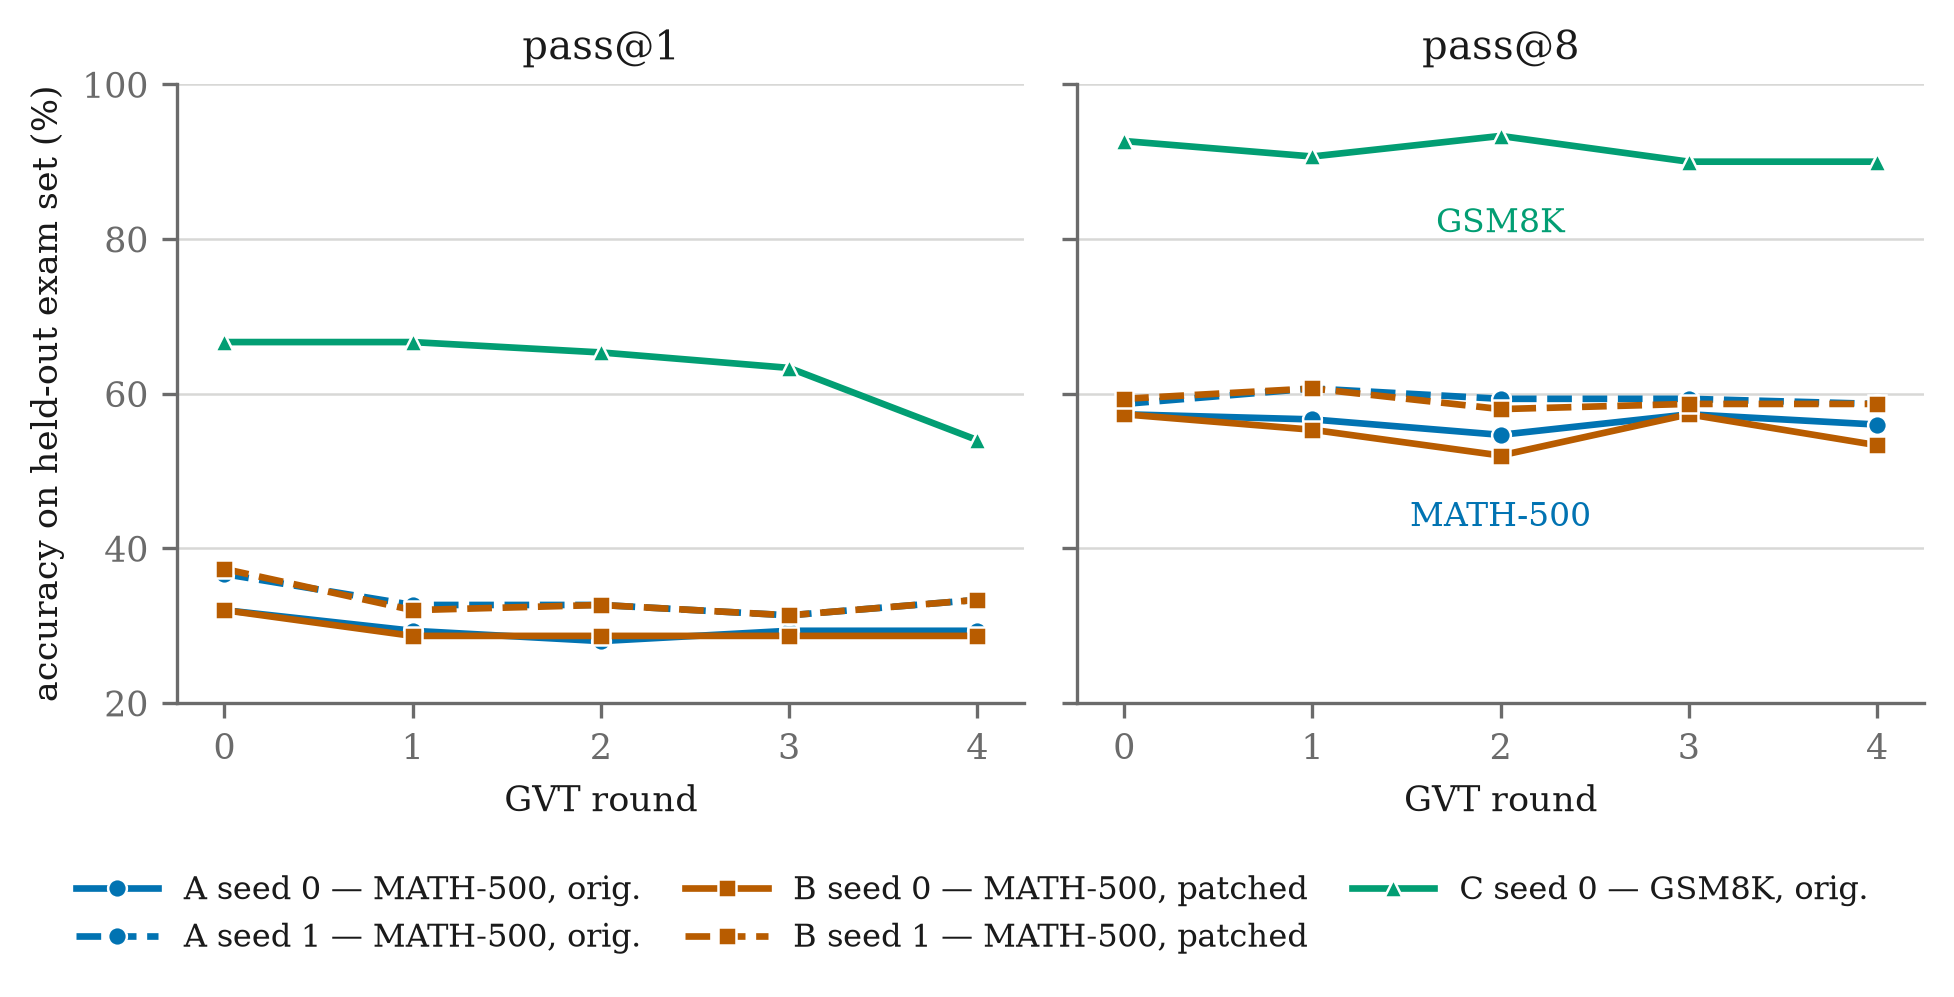
\includegraphics[width=\textwidth]{isolated_by_round.png}
\caption{Design~I at $10^{-5}$: pass@1 (left) and pass@8 (right) on the held-out
exam set, by round. Colour identifies the run, line style the seed, marker the
run again, so the figure survives greyscale printing. Runs A and B track each
other closely at both seeds. pass@8 stays within a few points in every run.
The one large visible movement is Run~C's pass@1 in the final round.}
\label{fig:isolated}
\end{figure}

\begin{table}[t]
\caption{Design~I: pass@1 and pass@8 on the held-out exam set (150
problems), Qwen2.5-1.5B, learning rate $10^{-5}$. Runs A and B differ only in the
\texttt{\textbackslash dfrac}/\texttt{\textbackslash tfrac} patch. Each seed draws its own exam partition, so
round-0 values differ between seeds.}
\label{tab:isolated}
\centering
\begin{tabular}{llccccc c}
\toprule
Run & Metric & R0 & R1 & R2 & R3 & R4 & $\Delta$ \\
\midrule
A, seed 0 (MATH-500, orig.) & pass@1 & 32.0\% & 29.3\% & 28.0\% & 29.3\% & 29.3\% & $-2.7$ pt \\
A, seed 0 (MATH-500, orig.) & pass@8 & 57.3\% & 56.7\% & 54.7\% & 57.3\% & 56.0\% & $-1.3$ pt \\
A, seed 1 (MATH-500, orig.) & pass@1 & 36.7\% & 32.7\% & 32.7\% & 31.3\% & 33.3\% & $-3.3$ pt \\
A, seed 1 (MATH-500, orig.) & pass@8 & 58.7\% & 60.7\% & 59.3\% & 59.3\% & 58.7\% & $\phantom{-}0.0$ pt \\
B, seed 0 (MATH-500, patched) & pass@1 & 32.0\% & 28.7\% & 28.7\% & 28.7\% & 28.7\% & $-3.3$ pt \\
B, seed 0 (MATH-500, patched) & pass@8 & 57.3\% & 55.3\% & 52.0\% & 57.3\% & 53.3\% & $-4.0$ pt \\
B, seed 1 (MATH-500, patched) & pass@1 & 37.3\% & 32.0\% & 32.7\% & 31.3\% & 33.3\% & $-4.0$ pt \\
B, seed 1 (MATH-500, patched) & pass@8 & 59.3\% & 60.7\% & 58.0\% & 58.7\% & 58.7\% & $-0.7$ pt \\
C, seed 0 (GSM8K, orig.) & pass@1 & 66.7\% & 66.7\% & 65.3\% & 63.3\% & 54.0\% & $-12.7$ pt \\
C, seed 0 (GSM8K, orig.) & pass@8 & 92.7\% & 90.7\% & 93.3\% & 90.0\% & 90.0\% & $-2.7$ pt \\
\bottomrule
\end{tabular}
\end{table}

\subsection{The Patch Control Could Not Detect an Effect}
\label{sec:control}
\label{sec:prevalence}
\label{sec:answer-diversity}

Runs A and B differ only in the \verb|\dfrac|/\verb|\tfrac| patch. At round~4,
B minus A is $-0.7$ [$-3.3$, $+2.0$] points of pass@1 at seed~0 and $+0.0$
[$-2.7$, $+2.7$] at seed~1. This null is uninformative: \verb|\dfrac| appears
in $0.50$--$0.73\%$ of generations, so the kept pools differ by $3$--$4$
examples (under $0.5\%$), and at $10^{-5}$ the adapter changes the outputs
little anyway. Removing one rare format defect had no detectable effect, which a
prevalence count alone predicts; the frequent gold-storage defect is present in
both arms. The pre-filter share of problems on which all $k$ samples agree falls
in every run, but it is mechanically tied to accuracy, so we draw no conclusion
from it (Appendix~\ref{app:control}).

\subsection{Higher Learning Rates}
\label{sec:lrcheck}

Because $10^{-5}$ changed the MATH-500 outputs little, we reran Run~A at
$10^{-4}$ (three seeds), $2\times10^{-4}$ (two) and $5\times10^{-4}$ (two,
with Run~B), with three rounds and $k=4$ (Table~\ref{tab:lrseries}).
\emph{At $5\times10^{-4}$ every run declines:} pass@1 falls $4.0$--$11.3$
points and the sample-accuracy intervals exclude zero in all four A/B runs,
though same-seed A and B are closer to two replicates than four.
\emph{The decline may grow with the rate on one seed:} at seed~1 sample accuracy
falls $1.5$, $3.5$ and $8.3$ points across the three rates, at seed~2 an almost
flat $3.7$, $3.8$ and $4.7$. The cap-hit share rises only at $5\times10^{-4}$.
\emph{The patch has no consistent effect:} B minus A in round-2 pass@1 is
$+5.3$ at seed~1 and $-7.3$ [$-14.0$, $-0.7$] at seed~2, a sign flip from pools
that differ by $0$--$3$ examples, which illustrates trajectory noise.
\emph{Style does not separate imitation from drift:} finished exam generations
start more boxed than the verifier-accepted pool and fall below it as the pool
falls too, which imitation of the pool and drift would both produce.

\begin{table}[t]
\caption{Run~A (MATH-500, original verifier, $k=4$, three rounds) across learning
rates and seeds: pass@1, pass@4 and sample accuracy (600 exam generations) at
round~0 $\to$ round~2, the share of round-2 generations that hit the
$512$-token cap (decoded text re-tokenised to $\ge508$ tokens; round~0 is
$43.0$--$43.2\%$, $48.2\%$ at seed~3), and problems added/lost summed over
rounds 1--2. The two $5\times10^{-4}$ rows are the A rows
of Table~\ref{tab:lrcheck}.}
\label{tab:lrseries}
\centering
\setlength{\tabcolsep}{3pt}
\begin{tabular}{llccccc}
\toprule
Rate & Seed & pass@1 & pass@4 & Sample acc. & Cap-hit (R2) & Added/lost \\
\midrule
$10^{-4}$ & 1 & $33.3\to34.0$ & $50.0\to49.3$ & $33.7\to32.2$ & $42.7\%$ & $20/21$ \\
$10^{-4}$ & 2 & $31.3\to28.0$ & $51.3\to45.3$ & $30.8\to27.2$ & $42.8\%$ & $25/34$ \\
$10^{-4}$ & 3 & $29.3\to26.7$ & $40.0\to41.3$ & $28.5\to27.5$ & $45.7\%$ & $16/14$ \\
$2\times10^{-4}$ & 1 & $33.3\to31.3$ & $50.0\to46.7$ & $33.7\to30.2$ & $40.8\%$ & $23/28$ \\
$2\times10^{-4}$ & 2 & $31.3\to25.3$ & $51.3\to45.3$ & $30.8\to27.0$ & $39.7\%$ & $21/30$ \\
$5\times10^{-4}$ & 1 & $33.3\to23.3$ & $50.0\to42.7$ & $33.7\to25.3$ & $46.2\%$ & $22/33$ \\
$5\times10^{-4}$ & 2 & $31.3\to27.3$ & $51.3\to44.7$ & $30.8\to26.2$ & $51.2\%$ & $26/36$ \\
\bottomrule
\end{tabular}
\end{table}

\begin{table}[t]
\caption{Change from round~0 to the last round (percentage points) with 95\%
paired problem-level bootstrap intervals over the 150 exam problems
($10{,}000$ resamples; \texttt{experiments/viec3/bootstrap\_ci.py}). Last round
is R4 at $10^{-5}$ ($k=8$) and R2 elsewhere ($k=4$). ``Finished, matched'' is
the last-round accuracy of generations below the $512$-token cap minus the
untrained model's accuracy on the same problem mix (Section~\ref{sec:anatomy};
$2{,}000$ resamples, \texttt{experiments/viec3/review\_cpu/capanat.py}). The
intervals do not include training-seed variance. Recomputed values match the
reported ones except six round values that differ by one problem
(Section~\ref{sec:config}), e.g.\ B, seed~1 at $10^{-5}$, whose round-4 pass@8
is $58.0\%$ against $58.7\%$; the matched column uses the separate re-scoring
described there.}
\label{tab:ci}
\centering
\scriptsize
\setlength{\tabcolsep}{1.5pt}
\begin{tabular}{lcccc}
\toprule
Run, seed & $\Delta$pass@1 & $\Delta$pass@$k$ & $\Delta$sample acc. & Finished, matched \\
\midrule
\multicolumn{5}{l}{\emph{Learning rate $10^{-5}$}} \\
A, 0 & $-2.7$ [$-9.3,4.0$] & $-1.3$ [$-8.0,5.3$] & $-2.4$ [$-4.8,0.0$] & $-3.8$ [$-7.2,-0.5$] \\
A, 1 & $-3.3$ [$-10.0,3.3$] & $+0.0$ [$-6.0,6.0$] & $-1.5$ [$-4.1,1.0$] & $-2.3$ [$-5.9,1.2$] \\
B, 0 & $-3.3$ [$-10.0,3.3$] & $-4.0$ [$-10.7,2.7$] & $-3.2$ [$-5.9,-0.6$] & $-4.2$ [$-7.8,-0.9$] \\
B, 1 & $-4.0$ [$-10.7,2.7$] & $-1.3$ [$-7.3,4.7$] & $-1.2$ [$-3.7,1.3$] & $-1.1$ [$-4.6,2.6$] \\
C, 0 & $-12.7$ [$-21.3,-4.0$] & $-2.7$ [$-7.3,2.0$] & $-13.1$ [$-16.7,-9.8$] & $-12.8$ [$-16.5,-9.4$] \\
\midrule
\multicolumn{5}{l}{\emph{Learning rate $10^{-4}$}} \\
A, 1 & $+0.7$ [$-6.7,8.0$] & $-0.7$ [$-6.0,4.7$] & $-1.5$ [$-5.3,2.2$] & $-4.3$ [$-9.6,1.1$] \\
A, 2 & $-3.3$ [$-9.3,2.7$] & $-6.0$ [$-12.7,0.7$] & $-3.7$ [$-7.3,-0.2$] & $-3.5$ [$-9.2,2.3$] \\
A, 3 & $-2.7$ [$-10.0,4.0$] & $+1.3$ [$-4.7,7.3$] & $-1.0$ [$-4.3,2.2$] & $-0.6$ [$-6.0,4.7$] \\
\multicolumn{5}{l}{\emph{Learning rate $2\!\times\!10^{-4}$}} \\
A, 1 & $-2.0$ [$-8.0,4.0$] & $-3.3$ [$-10.0,2.7$] & $-3.5$ [$-7.2,0.0$] & $-4.0$ [$-8.9,0.5$] \\
A, 2 & $-6.0$ [$-12.7,0.7$] & $-6.0$ [$-12.7,0.7$] & $-3.8$ [$-7.5,-0.2$] & $-4.7$ [$-10.1,1.0$] \\
\midrule
\multicolumn{5}{l}{\emph{Learning rate $5\!\times\!10^{-4}$}} \\
A, 1 & $-10.0$ [$-16.7,-3.3$] & $-7.3$ [$-14.0,0.0$] & $-8.3$ [$-12.3,-4.5$] & $-9.1$ [$-14.2,-4.2$] \\
A, 2 & $-4.0$ [$-11.3,3.3$] & $-6.7$ [$-13.3,0.0$] & $-4.7$ [$-8.2,-1.2$] & $-5.5$ [$-11.7,0.1$] \\
B, 1 & $-4.7$ [$-12.0,2.7$] & $-2.0$ [$-8.7,4.7$] & $-6.7$ [$-10.5,-2.8$] & $-6.8$ [$-12.4,-1.0$] \\
B, 2 & $-11.3$ [$-17.3,-5.3$] & $-11.3$ [$-18.0,-4.7$] & $-9.2$ [$-12.8,-5.5$] & $-5.9$ [$-10.9,-1.0$] \\
No filter, 1 & $-6.0$ [$-12.7,1.3$] & $-9.3$ [$-16.7,-2.7$] & $-8.2$ [$-12.2,-4.3$] & $-10.6$ [$-16.4,-5.5$] \\
No filter, 2 & $-8.7$ [$-16.0,-1.3$] & $-12.0$ [$-19.3,-4.7$] & $-10.2$ [$-14.2,-6.3$] & $-6.6$ [$-11.4,-2.0$] \\
Gold, 1 & $-18.0$ [$-26.7,-10.0$] & $-20.7$ [$-28.7,-12.7$] & $-19.7$ [$-25.3,-14.2$] & $-25.6$ [$-32.1,-18.9$] \\
Gold, 2 & $-21.3$ [$-28.7,-14.0$] & $-20.7$ [$-29.3,-12.7$] & $-18.7$ [$-23.7,-13.7$] & $-25.9$ [$-31.7,-20.0$] \\
C, 1 & $-22.0$ [$-29.3,-15.3$] & $-9.3$ [$-15.3,-3.3$] & $-15.3$ [$-19.8,-11.2$] & $-12.1$ [$-16.6,-7.9$] \\
\bottomrule
\end{tabular}
\end{table}

\paragraph{Two controls at $5\times10^{-4}$.}
The \emph{no-filter} run trains on all $k$ samples of every selection problem
($1{,}400$ examples per round), removing the verifier; the
\emph{train-on-gold} run trains on the $350$ reference solutions every round
(Table~\ref{tab:controls}). Neither is a single-variable control: no-filter
takes $3$--$4\times$ Run~A's optimizer steps, train-on-gold about the same.
Removing the filter is never better than keeping it beyond noise and is worse on
pass@4 at both seeds (round-2 differences $-2.0$ and $-5.3$ points, intervals
including zero), but the dose difference means this cannot be attributed to the
filter. Training on reference solutions is followed by a much larger decline
(pass@4 down about $21$ points at both seeds) while the model adopts the
reference style (\texttt{\$}-delimited spans $5\%\to98\%$); post hoc checks
suggest this fall is mostly real rather than verifier error. Run~C at
$5\times10^{-4}$ (GSM8K, one run) falls $22.0$ points of pass@1, from both less
accurate and more unfinished solutions (Appendix~\ref{app:lrcheck}).

\begin{table}[t]
\caption{Controls at $5\times10^{-4}$ (MATH-500, $k=4$, three rounds), on the
exam partition of Run~A at the same seed. Pool is the number of training
examples per round; optimizer steps are half of it.}
\label{tab:controls}
\centering
\setlength{\tabcolsep}{5pt}
\begin{tabular}{lccccccc}
\toprule
Run & Pool & \multicolumn{3}{c}{pass@1} & \multicolumn{3}{c}{pass@4} \\
 &  & R0 & R1 & R2 & R0 & R1 & R2 \\
\midrule
\multicolumn{8}{l}{\emph{Seed 1}} \\
A (verifier-filtered) & 440$\to$326 & 33.3 & 32.7 & 23.3 & 50.0 & 49.3 & 42.7 \\
No filter             & 1400 & 33.3 & 26.7 & 27.3 & 50.0 & 49.3 & 40.7 \\
Train on gold         & 350  & 33.3 & 18.0 & 15.3 & 50.0 & 33.3 & 29.3 \\
\midrule
\multicolumn{8}{l}{\emph{Seed 2}} \\
A (verifier-filtered) & 424$\to$350 & 31.3 & 31.3 & 27.3 & 51.3 & 46.0 & 44.7 \\
No filter             & 1400 & 31.3 & 34.7 & 22.7 & 51.3 & 48.7 & 39.3 \\
Train on gold         & 350  & 31.3 & 8.7 & 10.0 & 51.3 & 28.7 & 30.7 \\
\bottomrule
\end{tabular}
\end{table}

\subsection{Anatomy of the Decline}
\label{sec:anatomy}

This subsection is post hoc and descriptive. Sample accuracy mixes whether a
finished solution is right with whether the model finishes within the
$512$-token cap at all. Re-tokenising the saved text, we call a generation
\emph{cap-hit} at $\ge508$ tokens. The untrained model already hits the cap in
$41$--$48\%$ of MATH-500 generations, so the cap binds from the start. An
earlier character-length proxy for unfinished generations overstated
termination, because drifting prose crosses its threshold within the same token
budget. At $5\times10^{-4}$, compared with the untrained model on the same
problem mix, finished generations lose $5.5$--$10.6$ points, with intervals
excluding zero in five of six runs, while the cap-hit share rises $2$--$14$
points. A three-part decomposition attributes $12$--$30\%$ of the decline to the
cap share at seed~1 and $52$--$72\%$ at seed~2 (Table~\ref{tab:decomp}). At
$10^{-4}$ and $2\times10^{-4}$ the cap-hit share does not rise and finished
accuracy carries the whole change. Train-on-gold is different: responses
shorten by more than half and finished accuracy collapses. Retraining without
truncated examples and re-scoring adapters at a $1{,}536$-token cap leave the
picture unchanged, within the noise of single runs
(Appendix~\ref{app:anatomy}).

\begin{table}[t]
\caption{Decomposition of the change in sample accuracy (points, round~0 $\to$
last round, MATH-500 exam unless stated) into finished-accuracy, cap-share and
cap-accuracy parts, with the change in cap-hit share. Intervals: paired
problem-level bootstrap, $2{,}000$ resamples. The share is the finished part
over the whole change.}
\label{tab:decomp}
\centering
\scriptsize
\setlength{\tabcolsep}{2pt}
\begin{tabular}{lccccccc}
\toprule
Run, seed & $\Delta$cap-hit & $\Delta$acc. & Finished & Cap-share & Cap-acc. & Fin.\ share \\
\midrule
\multicolumn{7}{l}{\emph{$5\times10^{-4}$}} \\
A, 1 & $+3.0$ [$-1.7,7.7$] & $-8.3$ & $-6.0$ & $-1.3$ & $-1.0$ & $73\%$ [$43,108$] \\
B, 1 & $+4.7$ [$0.2,9.5$] & $-6.7$ & $-4.2$ & $-2.0$ & $-0.5$ & $62\%$ [$21,100$] \\
No filter, 1 & $+2.3$ [$-2.5,6.8$] & $-8.2$ & $-6.0$ & $-1.0$ & $-1.1$ & $74\%$ [$46,106$] \\
A, 2 & $+8.2$ [$3.8,12.3$] & $-4.7$ & $-2.7$ & $-3.4$ & $+1.5$ & $59\%$ [$-11,114$] \\
B, 2 & $+11.0$ [$6.2,16.0$] & $-9.2$ & $-3.6$ & $-4.8$ & $-0.8$ & $39\%$ [$6,64$] \\
No filter, 2 & $+14.2$ [$9.3,18.8$] & $-10.2$ & $-3.5$ & $-6.1$ & $-0.6$ & $34\%$ [$5,57$] \\
A replicate, 1 & $-0.2$ [$-4.5,4.3$] & $-5.2$ & $-4.6$ & $+0.1$ & $-0.7$ & $89\%$ [$41,162$] \\
A, 1024 limit, 1 & $+0.7$ [$-3.7,5.2$] & $-5.7$ & $-4.8$ & $-0.3$ & $-0.5$ & $85\%$ [$42,169$] \\
C (GSM8K), 1 & $+11.2$ [$7.8,14.7$] & $-15.3$ & $-7.8$ & $-6.6$ & $-0.9$ & $51\%$ [$30,66$] \\
\multicolumn{7}{l}{\emph{$2\times10^{-4}$ and $10^{-4}$}} \\
A, $2\times10^{-4}$, 1 & $-2.3$ [$-6.7,2.3$] & $-3.5$ & $-4.3$ & $+1.0$ & $-0.2$ & $124\%$ \\
A, $2\times10^{-4}$, 2 & $-3.3$ [$-7.7,1.0$] & $-3.7$ & $-5.2$ & $+1.4$ & $+0.1$ & $142\%$ \\
A, $10^{-4}$, 1 & $-0.5$ [$-4.5,3.7$] & $-1.8$ & $-3.1$ & $+0.2$ & $+1.0$ & $169\%$ \\
A, $10^{-4}$, 2 & $-0.2$ [$-4.3,4.0$] & $-3.7$ & $-3.4$ & $+0.1$ & $-0.3$ & $93\%$ \\
A, $10^{-4}$, 3 & $-2.5$ [$-6.3,1.3$] & $-1.0$ & $-1.4$ & $+1.1$ & $-0.7$ & $139\%$ \\
\bottomrule
\end{tabular}
\end{table}

\section{Discussion}
\label{sec:discussion}

\subsection{Answer to the Research Question}
\label{sec:answer}

\emph{Does the model get better at mathematics?} Not detectably. No run raises
pass@1 or pass@$k$ by an amount whose interval excludes zero, at any rate, and
the sample-accuracy intervals exclude gains above about $2.2$ points. The bound
is loose: it is read off observed intervals rather than a pre-specified
equivalence test, uses a measure chosen after the runs (on pass@1 and pass@$k$
the upper ends reach $+8.0$ and $+7.3$), and omits training-seed variance. In
every MATH-500 run but one, the problems lost equal or outnumber those gained.

\emph{Does it learn to write what the verifier accepts?} The data cannot settle
this. The pre-set pattern requires pass@1 to rise, which never happens
detectably (the largest rise is $+0.7$ [$-6.7$, $+8.0$]), so the rule's silence
is not evidence against verifier-style learning. The \verb|\boxed| share falls
in a way imitation and drift would both produce. The one direct test points away
from adaptation for one defect class: the share of correct answers the
gold-storage defect rejects does not fall over rounds.

\emph{What happened to the pooled collapse?} It does not reproduce when each
dataset has its own adapter and is scored on held-out problems. Because the
pooled design also trained on about $4.5\times$ more examples per round, we
cannot say whether pooling, selection-set scoring or dose produced it.

\subsection{Interpretation}
\label{sec:threevars}

An earlier version explained the Design~P curves by a self-reinforcing
shrinking pool shaped by the biased verifier. The data neither support nor rule
it out: the patch tests how strong a rare bias is, not whether a frequent bias
compounds; the no-filter control declines without any verifier but with more
dose. The defensible statement is narrow: \emph{removing a format defect present
in under $1\%$ of generations, or removing the filter entirely, made no
consistent difference at the resolution of this setup}. The frequent gold-storage
defect was never varied, so whether systematic false negatives are harmless in
general, as Egashira et al.\ find for RLVR, our data cannot say. Practical
suggestions are listed in Appendix~\ref{app:discussion}.

\section{Limitations}
\label{sec:limitations}

\emph{Unequal training doses} confound every cross-arm comparison.
\emph{The controls are underpowered:} the patch changes $0$--$4$ training
examples, and the no-filter and train-on-gold controls have two seeds each.
\emph{Intervals cover only problem draw and sampling,} not training-seed
variance; several conditions have one seed, and no multiplicity correction is
applied. \emph{The learning-rate grid is coarse,} with three rounds and $k=4$.
\emph{Cap-hit is reconstructed} from decoded text. \emph{The verifier audit} used
other models' solutions and inspected only rejections; the gold-storage defect
was measured afterwards and ran unvaried through every run, and the same
verifier both selects and grades. \emph{The $512$-token cap binds} from the
start. \emph{Scope:} one model size in Design~I, one verifier, one LoRA recipe
with loss over the prompt, a restart-from-base design that leaves compounding
little room, and possible test-set contamination. No arm improves on round~0,
so we have no positive reference showing this recipe can help a 1.5B model.
Appendix~\ref{app:limitations} gives the full list.

\section{Conclusion}
\label{sec:conclusion}

We asked whether generate--verify--select--train iterations make a 1.5B model
better at mathematics or only teach it to write what a rule-based verifier
accepts. On a held-out exam, the first answer is no: on the four measures fixed
in advance no run improves detectably, and the intervals for sample accuracy (a
primary measure chosen after the runs) exclude gains above about $2.2$ points,
a loose bound because they omit training-seed variance and are not an
equivalence test. The second stays open, because our pre-set rule for it could
only fire if accuracy rose, and the post hoc \verb|\boxed| share falls in a way
that imitation of the less-boxed training pool and drift would both produce. In
a post hoc description, most clearly at the highest rate, the model becomes less
accurate on the solutions it does finish; more generations
hit the token cap only at the highest rate, and clearly only at one of its two
seeds, where the change in cap-hit share accounts for $12$--$30\%$ of the
decline at seed~1 and $52$--$72\%$ at seed~2; a character-length heuristic we
first used overstated that part.
Reference-solution training degrades the model more, with much shorter answers.
Patching a rare verifier defect and removing the filter made no difference of
consistent sign across measures and seeds (pass@1 flips sign between seeds;
removing the filter lowers pass@4 at both seeds, within noise; single-seed
intervals sometimes exclude zero), neither control could have detected a small effect,
and a frequent defect in our gold storage, which rejects about one in six
correct solutions, ran unvaried through every experiment. A sharp
decline seen in an earlier pooled design does not reproduce under isolation and
held-out scoring, and because that design also trained several times longer per
round, we leave its cause open. We report the earlier readings that did not hold
up because the designs that produced them are common.

Future work, including a dose-matched control for the gold-storage defect,
is outlined in Appendix~\ref{app:future}.

\begin{credits}
\subsubsection{\ackname}
This work was carried out as an undergraduate research project. No external
funding was received.

\subsubsection{\discintname}
The authors have no competing interests to declare that are relevant to the
content of this article.
\end{credits}

\begin{thebibliography}{99}

\bibitem{ref_imperfect}
Cai, X.-Q., Wang, W., Liu, F., Liu, T., Niu, G., Sugiyama, M.:
Reinforcement Learning with Verifiable yet Noisy Rewards under Imperfect
Verifiers. arXiv:2510.00915 (2025)

\bibitem{ref_gsm8k}
Cobbe, K., Kosaraju, V., Bavarian, M., Chen, M., Jun, H., Kaiser, L.,
Plappert, M., Tworek, J., Hilton, J., Nakano, R., Hesse, C., Schulman, J.:
Training Verifiers to Solve Math Word Problems. arXiv:2110.14168 (2021)

\bibitem{ref_delayplateau}
Egashira, K., Vero, M., Dekoninck, J., D\"orner, F.E., Staab, R., Vechev,
M.: Delay, Plateau, or Collapse: Evaluating the Impact of Systematic
Verification Error on RLVR. arXiv:2605.02909 (2026)

\bibitem{ref_math}
Hendrycks, D., Burns, C., Kadavath, S., Arora, A., Basart, S., Tang, E.,
Song, D., Steinhardt, J.: Measuring Mathematical Problem Solving With the
MATH Dataset. arXiv:2103.03874 (2021)

\bibitem{ref_robustness}
Huang, Y., Zeng, W., Zeng, X., Zhu, Q., He, J.: From Accuracy to
Robustness: A Study of Rule- and Model-based Verifiers in Mathematical
Reasoning. arXiv:2505.22203 (2025)

\bibitem{ref_selfdistill}
Kim, J., Luo, X., Kim, M., Lee, S., Kim, D., Jeon, J., Li, D., Yang, Y.:
Why Does Self-Distillation (Sometimes) Degrade the Reasoning Capability of
LLMs? arXiv:2603.24472 (2026)

\bibitem{ref_selectionbias}
Qiao, X., Du, X., Liu, W., Zhang, J., Mai, P., Zhang, M., Pang, Y.:
When Sample Selection Bias Precipitates Model Collapse. arXiv:2606.13732
(2026)

\bibitem{ref_collapse}
Shumailov, I., Shumaylov, Z., Zhao, Y., Papernot, N., Anderson, R., Gal,
Y.: AI models collapse when trained on recursively generated data. Nature
(2024). \doi{10.1038/s41586-024-07566-y}

\bibitem{ref_restem}
Singh, A., Co-Reyes, J.D., Agarwal, R., et al.: Beyond Human Data: Scaling
Self-Training for Problem-Solving with Language Models. arXiv:2312.06585
(2023)

\bibitem{ref_rest}
Gulcehre, C., Le Paine, T., Srinivasan, S., et al.: Reinforced
Self-Training (ReST) for Language Modeling. arXiv:2308.08998 (2023)

\bibitem{ref_teacherfree}
Strozzi, I.L.: Teacher-Free Self-Training Amplifies but Does Not Compound:
A Pass@k Crossover on a Free-Verifier Domain. arXiv:2606.07856 (2026)

\bibitem{ref_phantom}
Xu, C., Yan, N., Chen, L., Kechadi, M.-T.: Phantom Gains: Auditing
Self-Improvement Against a Measured Null. arXiv:2608.20290 (2026)

\bibitem{ref_tinyv}
Xu, Z., Li, Y., Jiang, F., Ramasubramanian, B., Niu, L., Lin, B.,
Poovendran, R.: TinyV: Reducing False Negatives in Verification Improves RL
for LLM Reasoning. arXiv:2505.14625 (2025)

\bibitem{ref_rft}
Yuan, Z., Yuan, H., Li, C., Dong, G., Lu, K., Tan, C., Zhou, C., Zhou, J.:
Scaling Relationship on Learning Mathematical Reasoning with Large Language
Models. arXiv:2308.01825 (2023)

\bibitem{ref_rllimit}
Yue, Y., Chen, Z., Lu, R., Zhao, A., Wang, Z., Yue, Y., Song, S., Huang,
G.: Does Reinforcement Learning Really Incentivize Reasoning Capacity in
LLMs Beyond the Base Model? arXiv:2504.13837 (2025)

\bibitem{ref_star}
Zelikman, E., Wu, Y., Mu, J., Goodman, N.D.: STaR: Bootstrapping Reasoning
With Reasoning. arXiv:2203.14465 (2022)

\end{thebibliography}

\appendix

\section{Related Work in Full}
\label{app:related}

\paragraph{Self-training and its limits.}
STaR~\cite{ref_star} introduced the generate--filter--retrain loop, and
ReST~\cite{ref_rest}, ReST-EM~\cite{ref_restem} and RFT~\cite{ref_rft} formalise
it; ReST-EM, which like us restarts fine-tuning from the base model each
iteration, reports diminishing test gains after the first round and a one-round
regression on APPS. ReST filters machine-translation samples with a learned
reward model and a rising threshold; the others filter by answer correctness.
None of them measures how the filter's errors depend on the form of the answer,
and they mostly use larger models than ours. Yue et al.~\cite{ref_rllimit} show that RL
raises pass@1 while the base model wins at large pass@$k$, and Teacher-Free
Self-Training~\cite{ref_teacherfree} observes a pass@8 versus pass@64 crossover on
a free-verifier domain, concluding that self-training ``amplifies but does not
compound''. Training repeatedly on model-generated data erodes distribution
tails~\cite{ref_collapse}, and Qiao et al.~\cite{ref_selectionbias} argue
theoretically that a selector seeing only a narrow slice of the target
distribution accelerates collapse.

\paragraph{Verifier error.}
TinyV~\cite{ref_tinyv} measures that rule-based verifiers reject many correct
solutions and repairs them with an LLM check. From Accuracy to
Robustness~\cite{ref_robustness} reports an average recall of $86\%$ for
rule-based verifiers, i.e.\ about $14\%$ of correct responses rejected, but for
\texttt{math-verify} itself on their MATH subset a recall of $0.95$ (about $5\%$
false negatives; their Table~5, on DeepSeek-R1-Distill-Qwen-32B outputs). Our
MATH-500 audit gives $7.8\%$ (95\% Wilson interval $4.3$--$13.8\%$) on another
model's solutions, a figure whose relation to the loop's own rate is not known
(Section~\ref{app:verifier}), and a pipeline-specific defect alone rejects
$15.5$--$18.4\%$ of the loop's own solutions that a repaired verifier accepts. These figures differ in
verifier version, solution source and denominator, so we compare them only in
order of magnitude. Imperfect Verifiers~\cite{ref_imperfect} gives the most formal noise model,
with fixed false-accept and false-reject probabilities, and notes that real noise
can depend on formatting but then assumes content-independent rates. Egashira et
al.~\cite{ref_delayplateau} classify verifier errors in RLVR on a synthetic
arithmetic task (Qwen3-1.7B-Base and OLMo3-7B, with Qwen2.5-1.5B-Instruct, our
model, in an appendix) with hand-designed patterns such as format-based false
negatives, and find that systematic false negatives behave like random noise
whereas false positives (rewards given to answers that are near the truth, or
that contain a keyword) can cause plateau or collapse; they also note that a
domain whose queries are always rejected can at best plateau, which is the
position of our unparseable-gold problems. Our
setting differs in paradigm (offline rejection-sampling SFT with a fresh adapter
per round, not on-policy RL) and in task (real benchmark problems). Our patch
control cannot test their false-negative finding, because it changes too little
of the training pool (Section~\ref{app:control}), and the much larger
false-negative class we measured afterwards is present in both arms. Nor does
our no-filter control test their false-positive finding: their false positives
are systematic (a fixed wrong pattern that is always accepted), whereas
no-filter admits every sample, about two thirds of them incorrect in
unstructured ways, under SFT with a $3$--$4\times$ larger training dose. It did
not end consistently worse than the filtered run, which we report only as a
related observation.

\paragraph{Auditing self-improvement.}
Xu et al.~\cite{ref_phantom} audit three rounds of rank-32 LoRA self-training of
Qwen3-8B ($\eta=10^{-4}$; filters by answer match or majority vote, plus a
distillation arm from an external teacher as a positive control) against a
frozen untrained control, and identify seven measurement failures that each
invert a reported finding when its control is absent, including training-seed
variance and a fixed token cap under style drift: their distillation arm, the
most effective one, scored as the most destructive because its truncation rate
rose from $16.5\%$ to $65.3\%$.
Self-training does not improve rarely-solved problems and corrupts problems
solved at baseline. This is the study closest to ours in spirit. Our per-problem
added/lost counts point the same way (more problems lost than gained), though
without their frozen control and with net counts that only restate the change
in pass@$k$ (Section~\ref{sec:config}), and our
adapters also drift in style (longer outputs, fewer \verb|\boxed| answers), and
a fixed token cap matters in our setting too: the untrained model already hits
it in $41$--$48\%$ of MATH-500 generations. Their finding is a warning that a
decline under a fixed cap can be misread as lost capability; this is why we
separate finished accuracy from termination and re-score at a larger cap
(Section~\ref{app:anatomy}). Their setup differs in model size, rank and filters; we lack their
per-round frozen arm (we re-score the untrained model once,
Section~\ref{app:anatomy}) and a distillation arm, and we add a measured
format-biased verifier, a learning-rate series and reference-solution and
no-filter controls.

\paragraph{Reference-guided training.}
{\sloppy Kim et al.~\cite{ref_selfdistill} show that self-distillation conditioned on the
ground-truth solution can cut mathematical accuracy by up to $40\%$ (Qwen3-1.7B/8B,
DeepSeek-Distill-Qwen-7B and Olmo3-7B-Instruct) while \emph{shortening} responses,
which they trace to suppressed epistemic verbalization. Our train-on-gold control
is plain SFT on human reference solutions, not self-distillation, so it is at
most a loose analogue; it shows a similar surface signature (shorter responses,
lower accuracy) that may simply come from imitating terse references. We did not
measure epistemic markers.\par}

\paragraph{Positioning.}
In the literature we surveyed (searched through October 2026) we found no
multi-round self-training study that uses a rule-based verifier with a measured
format bias together with a matched patched-verifier control; the
closest are Egashira et al.\ and Xu et al. Given that the patch turned out to be
too weak to test anything (Section~\ref{app:control}), we do not present this
combination as the contribution. The contribution is the absence of a
detectable gain under four pre-set measures with intervals, the
description of what training at higher rates changes, and the design lessons.
\section{The Verifier in Full}
\label{app:verifier}

\emph{Format probe.} We re-rendered gold answers from GSM8K and MATH-500 in
individually valid formats (bare number, trailing-zero decimal, \verb|\frac|,
\verb|\dfrac|, \verb|\tfrac|, boxed, dollar-delimited, sentence, with units) and
asked the verifier to grade them against the original gold. On GSM8K plain
rewrites are never rejected, while \verb|\dfrac|/\verb|\tfrac| are rejected
$200/200$ (the command is not parsed). On MATH-500, \verb|\dfrac|/\verb|\tfrac|
are rejected $146/146$ ($100\%$), trailing-zero decimals $13/22$, and boxed forms
$41/200$. Of those $41$, $24$ are gold answers our pipeline stores in forms the
verifier cannot parse at all, so part of this figure measures our gold storage,
not the verifier. The other $17$ ($17$ of the $200$ boxed probes, $8.5\%$) are
compound answers such as $3\sqrt{13}$: the gold is stored without a delimiter,
and \texttt{math-verify} applies its full \LaTeX{} extraction only inside
\verb|\boxed{}| or \verb|$...$|, so the bare gold is parsed to its first number
and no longer matches a correct boxed prediction.

\emph{False-negative rate on real solutions.} We took one public solution per
problem for the first $200$ problems of each dataset (teacher traces for GSM8K,
Qwen2.5-7B-Instruct rollouts for MATH-500), not the 1.5B model's own outputs.
Correctness was established by a scripted comparison of the boxed answer with
the gold string after normalisation (\texttt{src/dacntt/read.py}: delimiters,
braces, spaces and commas removed, \verb|\dfrac|/\verb|\tfrac| read as
\verb|\frac|, simple fractions compared by value), and we then counted how many of
these correct solutions the verifier rejects. The false-negative rate is
$7.8\%$ on MATH-500 ($10$ of $128$ correct solutions; $24$ problems with
unparseable gold excluded) and $0\%$ on GSM8K ($0/200$; 95\% Wilson interval
$0$--$1.9\%$, one-sided upper bound $1.3\%$), identical for the \texttt{default}
and \texttt{reward} extraction presets of \texttt{math-verify}. Of the ten
MATH-500 cases, eight are rejected when the whole solution is verified but
accepted when only the boxed answer is, which we labelled wrong-token
extraction from a long solution, and two are rewrites the normalisation
equates but the verifier does not match (e.g.\ \verb|6 + 9i| for \verb|6+9i|).
Most of the eight are compound answers ($3\sqrt{13}$, $6-5i$, $11\sqrt2$, a
list, a polynomial), so they overlap with the compound class of the format
probe; the two labels describe where the failure shows, not exclusive causes.
The $7.8\%$ estimates the false-negative rate on Qwen2.5-7B-Instruct solutions
for problems whose gold the verifier can parse, among answers our normalisation
recognises as correct. Correct answers in forms it does not equate are left out
of the denominator, and the $24$ problems with unparseable gold are counted as a
separate defect below; relative to the loop's own rate, where the 1.5B model
writes longer and, after training, less boxed solutions, the direction of the
difference is not known. The audit also inspected only rejected solutions, so it cannot measure
the false-positive rate; that the verifier rarely accepts wrong answers is an
assumption here, not a measurement.

\emph{Unparseable gold in the loop.} Over all $500$ MATH-500 problems the
verifier cannot parse $51$ stored gold answers ($10.2\%$); $11$--$18$ of them fall
in each $150$-problem exam partition. The loop keeps these problems: every
sample is rejected, so they never enter the training pool and always count as
unsolved. They lower absolute pass rates by up to $12$ points but are constant
within a partition, so they cancel in within-run and same-partition
comparisons. Wrapping the gold in \verb|\boxed{}|, the re-score described
below, makes $46$ of these $51$ golds parseable, so the two corrections overlap
and should not be added (\path{experiments/viec3/review_cpu/dot4/unparsed.py}).

\emph{The patch.} For the control we repaired the most \emph{severe} identified
failure mode with a normalisation pass that rewrites \verb|\dfrac| and
\verb|\tfrac| to \verb|\frac| before parsing, removing the $100\%$-rejection class
and nothing else. The patched verifier is therefore still biased: it keeps the
wrong-token extractions (8 of the 10 audited false negatives) and the
gold-storage defect.

\emph{The gold-storage defect in the loop's own outputs (post hoc).} After the runs we
re-scored the saved generations with a second normalisation that wraps the gold
in \verb|\boxed{}| when the prediction contains one and the gold does not
(\path{experiments/viec3/review_cpu/}: \texttt{patch\_dose.py},
\texttt{dose.py}, \texttt{flips.py}). This defect is far more frequent than the \verb|\dfrac|
class. Over all $500$ problems it rejects $15.5$--$18.4\%$ of the generations
the re-scored verifier accepts (Run~A at $5\times10^{-4}$, seeds~1 and~2, and
at $10^{-5}$, seed~0, every round). The kept pool covers only the $350$
selection problems, where the share is about the same ($17.8$--$18.8\%$ at round~0): accepting these
generations would enlarge the round-0 pool by about a fifth (Run~A at seed~1:
$440\to542$, $+23\%$; at $10^{-5}$: $872\to1{,}066$, $+22\%$), against $0$--$4$
examples (under $1\%$) for the \verb|\dfrac| patch. In a hand
check of $30$ random flips, $29$ pairs were the same value written differently
(e.g.\ \verb|\frac43| and \verb|\frac{4}{3}|; one prediction had an empty box).
The $15.5$--$18.4\%$ assumes that the re-scored verifier itself accepts no wrong
answer, which we did not measure. On the exam set the defect lowers absolute
pass@1 by $6.7$--$8.0$ points at round~0 and throughout the $10^{-5}$ runs, by
$4.7$ points at round~2 under $5\times10^{-4}$, and by $0.7$--$3.3$ points for
train-on-gold after round~0. The absolute offset is therefore not constant, but
as a share of re-scored pass@1 it roughly is ($6.7/40.0$ and $4.7/28.0$, both
$17\%$, for Run~A at seed~1; $20\%$ throughout at $10^{-5}$): the defect rejects
about the same fraction of correct answers in every round, and the absolute
offset shrinks because accuracy falls. Two consequences follow. With the original
verifier the declines below are \emph{understated}, by a factor of about $0.73$--$0.78$
(the ratios of original to re-scored sample-accuracy changes below), and the
same factor shrinks every original-verifier difference and interval, including
the $2.2$-point bound on gains, which on the re-scored scale is nearer $3$
points. And the fraction of correct answers this defect rejects does not fall
over the rounds, so for this one defect class the model does not learn to avoid
what the verifier rejects; this is the only direct test of verifier adaptation
we have, and it covers one defect. We keep the original verifier's numbers in
every table, since that is the verifier the loop trained with; they are
therefore $4.7$--$8.0$ points too low in absolute terms for self-training. Re-scored, with paired bootstrap intervals as in Section~\ref{sec:config},
sample accuracy changes by $-10.7$ [$-14.8$, $-6.7$] and $-6.0$ [$-9.7$, $-2.2$]
points for Run~A at $5\times10^{-4}$ (seeds~1 and~2; original verifier $-8.3$
and $-4.7$), by $-3.3$ [$-5.9$, $-0.7$] for Run~A at $10^{-5}$, seed~0 (original
$-2.4$), and by $-24.7$ and $-22.0$ for train-on-gold. In pass@1 the same runs go
from $40.0\%$ to $28.0\%$ and from $38.0\%$ to $32.0\%$ (interval $[-14.0,+2.0]$
for the latter), from $40.0\%$ to $36.7\%$, and from $40.0\%$ to $16.0\%$ and
from $38.0\%$ to $13.3\%$. Only these five runs were re-scored, three of them
self-training; that the other runs' declines would also survive a re-score is
an extrapolation from these three. Both arms of the patch control
(Section~\ref{app:control}) carry this defect.
\section{Uncertainty in Full}
\label{app:uncertainty}

\paragraph{Uncertainty.} For every within-run change (round~0 against the last
round) and every paired comparison of two runs on the same exam partition we
report a 95\% interval from a paired problem-level bootstrap: we resample the
$150$ exam problems with replacement ($10{,}000$ times), recompute the statistic
for both rounds or runs on the same resampled problems, and take the 2.5th and
97.5th percentiles. Resampling problems rather than samples respects the
clustering of the $k$ samples within a problem. The per-sample correctness was
recomputed from the saved generations with the same verifier; it reproduces
the reported pass rates except for six round values that differ by one problem
($0.6$--$0.7$ points), most likely because of \texttt{math-verify} comparison
timeouts
(\texttt{experiments/viec3/bootstrap\_ci.py}). The post hoc measures of
Section~\ref{app:anatomy} (Table~\ref{tab:anatomy}, the matched column of
Table~\ref{tab:ci} and the decomposition) use a separate re-scoring of the same
generations (\texttt{review\_cpu/scored/}), which differs from the values behind
Tables~\ref{tab:lrseries} and~\ref{tab:ci} by up to one problem in some further
rounds (e.g.\ $10^{-4}$, seed~1, round~2: pass@1 $33.3$ against $34.0\%$); no
conclusion depends on these differences. These intervals cover the
choice of problems and the sampling of generations for a given trained adapter;
they do \emph{not} cover training-seed variance, which we can only see
informally across our two or three seeds, so they understate the uncertainty of
run-level conclusions. Our own data suggest by how much: a replicate of Run~A
at $5\times10^{-4}$, seed~1, with the same configuration, ends $3.2$ points of
sample accuracy away from the original (Section~\ref{app:anatomy}); and at
seed~2 Runs A and B, whose round-0 training pools are identical ($424$
examples each), end $7.3$ points apart in round-2 pass@1 (interval
$[-14.0,-0.7]$, Section~\ref{app:lrcheck}), though that is a single interval
near zero. A single interval that excludes zero is therefore not sufficient
evidence of a reproducible effect, and one that includes zero does not rule an
effect out. We also make no correction for multiplicity: Table~\ref{tab:ci}
alone holds $76$ intervals and the text about ten more, and at the 95\% level
about four of the $76$ would exclude zero by chance if nothing changed (fewer
or more, since they are not independent), so we rest conclusions on patterns
across runs and seeds, not on any single interval. Single proportions use Wilson intervals.

\section{Design P in Full}
\label{app:pooled}

\begin{table}[t]
\caption{The two designs. They differ in more than the intended variables;
the most quantifiable unintended difference is the training dose per round
(about $4.5\times$ as many optimizer steps in Design~P).}
\label{tab:designs}
\centering
\begin{tabular}{lll}
\toprule
& Design~P (pooled) & Design~I (isolated) \\
\midrule
Datasets per run & GSM8K + MATH-500 & one only \\
Adapter & one, shared & one per dataset \\
Training mixture & $\approx$\,69\% GSM8K & single-domain \\
Evaluation items & same as selection & held-out 30\% \\
Training examples, round 0 (1.5B) & $3{,}962$ & $872$ (A), $1{,}901$ (C) \\
Verifier control & none & Run~B (patched) \\
Models & 0.5B and 1.5B & 1.5B \\
\bottomrule
\end{tabular}
\end{table}

Table~\ref{tab:passk} reports pass@1 and pass@8 for both models over five rounds
of the pooled design, as computed during the run (where the two verifier
presets gave identical pooled values; a later per-dataset recomputation differs
by one problem, see Table~\ref{tab:bydataset}). The
1.5B decline is severe and accelerating; the 0.5B decline is small ($-3.7$ and
$-5.6$ points). Splitting the 1.5B run by dataset (Table~\ref{tab:bydataset})
shows both datasets falling heavily, although GSM8K has a measured $0\%$
false-negative rate, though that rate was measured on external solutions in
the untrained model's style, not on Design~P's late-round outputs. The accepted
pool also contracts every round (1.5B: $3{,}962$, $3{,}730$, $3{,}395$,
$2{,}638$, $1{,}566$; 0.5B: $2{,}533$ to $2{,}123$;
\path{experiments/viec3/review_cpu/dot4/poolP.py}) and the 1.5B output style shifts, with
\verb|\boxed{}| falling from $5{,}608$ to $2{,}693$ of $8{,}000$ generations while
dollar-delimited math rises from $1{,}453$ to $3{,}406$.


\begin{table}[t]
\caption{Design~P, 1.5B, split by dataset, recomputed from the saved
generations (preset \texttt{reward}, the one used for selection; the
\texttt{default} preset differs only at MATH-500 round-3 pass@8, $45.0\%$).
Pooled, the recomputed round-3 pass@8 is $63.5\%$ (\texttt{reward}) and
$63.6\%$ (\texttt{default}), against $63.6\%$ in Table~\ref{tab:passk}.}
\label{tab:bydataset}
\centering
\begin{tabular}{llccccc c}
\toprule
Dataset & Metric & R0 & R1 & R2 & R3 & R4 & $\Delta$ \\
\midrule
GSM8K & pass@1 & 69.6\% & 62.0\% & 61.0\% & 45.6\% & 26.6\% & $-43.0$ pt \\
GSM8K & pass@8 & 91.4\% & 90.4\% & 89.0\% & 82.2\% & 65.8\% & $-25.6$ pt \\
MATH-500 & pass@1 & 30.4\% & 30.4\% & 28.0\% & 19.2\% & 10.6\% & $-19.8$ pt \\
MATH-500 & pass@8 & 53.8\% & 52.6\% & 51.4\% & 44.8\% & 31.4\% & $-22.4$ pt \\
\bottomrule
\end{tabular}
\end{table}

Design~P cannot be interpreted causally, for three reasons. First, each round
trains one adapter on the union of both datasets' accepted solutions, of which
GSM8K supplies $68.4$--$70.2\%$ in every round, so either dataset's trajectory is
a joint function of both pools. Second, it scores each round on the problems it
also used to select training data. We expected this to \emph{raise} later-round
scores, if anything. Design~I lets us check that expectation, since it also
generates on its $350$ selection problems: there, Run~A's sample accuracy on the
selection problems falls as much as or more than on the exam at the two higher rates (e.g.\ Run~A at
$5\times10^{-4}$: $-8.2$ and $-5.3$ points against $-8.3$ and $-4.7$ on the
exam; at $10^{-4}$, seed~1: $-6.2$ against $-1.5$; no intervals); at
$10^{-5}$ it falls slightly less ($-1.0$ and $-1.1$ against $-2.4$ and $-1.4$),
and Run~C's selection problems fall less at $5\times10^{-4}$ ($-11.3$ against
$-15.4$) and slightly more at $10^{-5}$ ($-13.8$ against $-13.0$). Training on a problem's own accepted solutions therefore
did not protect it, so selection-set scoring is unlikely to have masked a
decline; since the selection problems sometimes fall more, it may have
enlarged one, and it remains a candidate contributor. Third, and not anticipated when we designed the follow-up, Design~P
trains on far more examples per round: $3{,}962$ at round~0 for the 1.5B model,
against $872$ for the isolated MATH-500 run at the same learning rate. With one
epoch and the same batch size this is about $4.5\times$ as many optimizer steps
(Design~P's training logs were not saved, so this is inferred from pool size).
Section~\ref{app:lrcheck} suggests, on the evidence of one seed, that a higher
learning rate produces more decline, with a falling \verb|\boxed| share as here
(pass@1 falls faster than pass@$k$ in only two of its four runs at
$5\times10^{-4}$), and Run~C, which takes about twice Run~A's steps per round
at the same rate, is the one $10^{-5}$ run that declines clearly. One reading
consistent with these data is that Design~P's adapter changed the model more.
It rests on two assumptions we have not tested: that more optimizer steps act
like a higher learning rate, and that Run~C's decline comes from its dose
rather than its dataset (a single comparator). Dose also explains at most the
level of the decline, not its time course: with a fresh adapter each round,
the round-$t$ model is trained on the round-$(t-1)$ pool alone, and the pools
shrink, yet the largest pass@1 drops ($-12.1$ and $-13.8$ points) come from the
two smallest pools ($3{,}395$ and $2{,}638$). Something carried through the
data, such as pool composition or style, fits this acceleration better. The
0.5B model, trained on $2{,}533$ examples at round~0 (about $2.9\times$ Run~A),
declines only a little, though it is a different model. Pooling or scoring may
also have contributed; no run separates these explanations.
\section{Design I at $10^{-5}$ in Full}
\label{app:isolated}

Table~\ref{tab:isolated} reports the isolated runs on their held-out exam sets.
pass@8 ends within $4$ points of its round-0 value in every run. On MATH-500,
pass@1 is $2.7$--$5.3$ points lower at round~1 than at round~0 and roughly flat
afterwards, and $2.7$--$4.0$ points lower at round~4; the bootstrap intervals for
these round-0-to-round-4 changes are between $[-10.7,+2.7]$ and $[-9.3,+4.0]$,
all including zero (Table~\ref{tab:ci}). With one first-sample draw per problem
per round, a step at round~1 cannot be distinguished from noise around a flat or
slightly negative trend, so we claim only that there is no evidence of
compounding on MATH-500 at this rate (Run~C, below, loses most of its pass@1 in
its last round), not that the first round has a one-off cost. The less
noisy measures do move: sample accuracy falls by $1.2$--$3.2$ points in these
four runs, with one interval (B, seed~0) excluding zero, and the (post hoc)
matched finished accuracy falls by $1.1$--$4.2$ points, with intervals excluding
zero at seed~0 for both A and B. These seed-0 intervals only just exclude zero
(upper ends $-0.6$ and $0.0$ for sample accuracy, $-0.5$ and $-0.9$ matched), A
and B at seed~0 share their round-0 generations and almost all of their first
pool, so they are close to one replicate, and at seed~1 nothing excludes zero.
With about four of the $76$ intervals in Table~\ref{tab:ci} expected to exclude zero by chance, we
read this as a possible small decline at this rate, not an established one;
what we do not see is a gain. Run~C (GSM8K)
declines more: pass@1 falls $12.7$ points, $9.3$ of them in the final round
($63.3\%\to54.0\%$; interval for the whole change $[-21.3,-4.0]$), and sample
accuracy $13.1$ points, while pass@8 falls $2.7$ points (interval including
zero) and the cap-hit share rises only from $3.5\%$ to $4.2\%$. Finished
accuracy falls $12.8$ points matched, and the decomposition of
Section~\ref{app:anatomy} puts $97\%$ of the sample-accuracy decline in finished
accuracy, so this decline is not a termination effect. It is a single run, and
it took about twice as many optimizer steps per round as Run~A ($951$ against
$436$ at round~0), so we do not attribute it to the dataset alone.


\paragraph{How much training happened at $10^{-5}$.}
The training loss does fall at this rate: within round~0 of Run~A it goes from
$0.72$ to $0.38$ (seed~0) and from $0.70$ to $0.40$ (seed~1) over about $420$
steps, with an epoch mean of $0.47$, against epoch means of $0.24$--$0.30$ at
$10^{-4}$--$5\times10^{-4}$. The adapter therefore learns, but slowly, and it
changes the outputs little: mean length and the share of generations that hit
the token cap are essentially unchanged from round~0 to round~4 (cap-hit
$46.9\to47.4\%$ at seed~0 and $40.7\to41.8\%$ at seed~1 for Run~A;
Table~\ref{tab:anatomy}). This holds for the MATH-500 runs at about $420$--$436$
steps per round; Run~C at the same rate, with about twice the steps, does
change its outputs. ``Little change'' is therefore a property of rate and
steps together, not of the rate alone. A flat pass@$k$ curve in the MATH-500
runs is evidence that this training step did little, not evidence that GVT is
stable.

\paragraph{Noise.}
Round~0 is the untrained base model, so round-0 differences between seeds
mostly measure how hard each partition is: round-0 pass@1 is $32.0\%$ at
seed~0 and $36.7\%$ at seed~1, and on the third partition used later round-0
pass@4 is $40.0\%$ against $50.0\%$ and $51.3\%$ on the other two
(Table~\ref{tab:lrseries}). These levels cancel in within-run changes. Noise in
the changes themselves is better seen elsewhere: re-sampling the same model on
the same problems moves pass@1 by up to $6.7$ points
(Section~\ref{app:anatomy}), and a single 150-problem pass@1 has a standard
error of about $3.8$ points. Agreement across seeds tests partition and
training variance together; training variance alone is seen only in
same-partition pairs (A against B at the same seed, Section~\ref{app:lrcheck},
and the replicate of Section~\ref{app:anatomy}). We therefore report the
bootstrap intervals above rather than judge differences against one ``noise
floor''.
\section{Patch Control and Answer Diversity in Full}
\label{app:control}

Runs A and B are identical in dataset, seed, split, model and training
configuration and differ only in whether \verb|\dfrac|/\verb|\tfrac| are
normalised before verification. Their curves are close
(Table~\ref{tab:isolated}): at round~4, B minus A is $-0.7$ [$-3.3$, $+2.0$] points of
pass@1 at seed~0 and $+0.0$ [$-2.7$, $+2.7$] at seed~1 (95\% intervals). Run~B's
exam is graded with the patched verifier, so these differences also contain a
grading offset: at seed~1 the identical round-0 generations already score
$0.6$ points higher in B, so the model part of the seed-1 difference is about
$-0.6$. Narrow intervals here bound the difference between two nearly identical
trajectories, not a patch effect. This null is uninformative, for two reasons
we should have checked before running it. First,
the treatment is tiny: \verb|\dfrac| appears in $20$--$29$ of the $4{,}000$
generations per round ($0.50$--$0.73\%$), \verb|\tfrac| never, and only the
correct ones among those are wrongly discarded; the kept pools of A and B differ
by $4$ examples at seed~0 ($872$ vs $876$) and $3$ at seed~1 ($833$ vs $836$),
under $0.5\%$ of the pool. Second, at $10^{-5}$ and the step count of these
MATH-500 runs the adapter changes the outputs little (Section~\ref{app:isolated}), so two nearly identical pools would give
nearly identical models whatever the verifier did. We cannot separate these
two explanations. The result is therefore: \emph{removing one rare format defect
had no detectable effect}, which the prevalence count alone predicts; it is not
evidence about directional verifier bias in general, and it leaves untouched the
gold-storage defect, which rejects $15.5$--$18.4\%$ of correct in-loop solutions
in both arms (Section~\ref{app:verifier}). Verifier-bias figures in
the literature, such as the $\sim$14\% of~\cite{ref_robustness}, are likewise
conditional on a reference distribution; what matters for a loop is how often
the affected forms occur in that loop's own output, which is cheap to count.

\paragraph{Pre-filter answer diversity.}
Over all problems of each run (in Design~I the $500$ selection and exam items
together, not the exam alone) we also measured, before filtering, the fraction of
problems on which all $k=8$ samples give the same extracted answer, for
Design~P's 1.5B run and the $10^{-5}$ Design~I runs at seed~0. It falls in
every one: $24.8\%\to1.7\%$ for Design~P's 1.5B
run, $33.6\%\to16.0\%$ for Run~C, $14.6\%\to12.0\%$ (A) and $14.6\%\to12.2\%$
(B). This agreement is mechanically tied to accuracy (problems on
which every sample is correct are all-agreement problems) and to generations
that hit the token cap, so it adds little beyond the accuracy change and does not by itself
rule out stylistic convergence, which concerns how answers are written rather
than which answer is given. The fraction of distinct answers among the $k$
samples, which we had planned as the primary diversity measure, barely moves at
$10^{-5}$ in the MATH-500 runs ($0.542\to0.554$ for Run~A, seed~0; $0.528\to0.543$
for Run~B, seed~1) but rises for Run~C ($0.359\to0.500$) and in Design~P
($0.443\to0.712$). We report both for completeness
and draw no conclusion from them.

\section{Higher Learning Rates in Full}
\label{app:lrcheck}

Because $10^{-5}$ changed the MATH-500 outputs little, we reran the MATH-500 runs at
higher rates with a smaller budget (three rounds, $k=4$, so pass@4 replaces
pass@8 and the pools are about half as large): Runs~A and B at $5\times10^{-4}$
at two seeds, and Run~A at $10^{-4}$ at three seeds and at $2\times10^{-4}$ at
two. Seed~1 shares the exam partition of the seed-1 runs above and seeds 2 and 3
draw new ones. These runs are not directly comparable with the $k=8$, five-round
runs in metric or training dose. Within round~0 the loss falls from about $0.5$
to $0.25$ at $5\times10^{-4}$ and from about $0.6$ to $0.28$ at $10^{-4}$ over
about $220$ steps.

\begin{table}[t]
\caption{Runs A and B at $5\times10^{-4}$ (MATH-500, $k=4$, three rounds),
held-out exam set of 150 problems. B differs from A only in the verifier patch;
each seed draws its own exam partition. ``Kept pool'' is the number of
training examples ($=2\times$ optimizer steps). ``Boxed'' is the share of the
$2{,}000$ generations in each round containing \texttt{\textbackslash boxed}.}
\label{tab:lrcheck}
\centering
\setlength{\tabcolsep}{6pt}
\begin{tabular}{lcccccc}
\toprule
Run, seed & Round & pass@1 & pass@4 & Kept pool & Boxed \\
\midrule
A (orig.), 1   & 0 & 33.3\% & 50.0\% & 440 & 52\% \\
               & 1 & 32.7\% & 49.3\% & 391 & 51\% \\
               & 2 & 23.3\% & 42.7\% & 326 & 36\% \\
B (patched), 1 & 0 & 33.3\% & 50.7\% & 443 & 52\% \\
               & 1 & 35.3\% & 50.0\% & 392 & 49\% \\
               & 2 & 28.7\% & 48.7\% & 328 & 41\% \\
\midrule
A (orig.), 2   & 0 & 31.3\% & 51.3\% & 424 & 54\% \\
               & 1 & 31.3\% & 46.0\% & 386 & 50\% \\
               & 2 & 27.3\% & 44.7\% & 350 & 37\% \\
B (patched), 2 & 0 & 31.3\% & 52.0\% & 424 & 54\% \\
               & 1 & 31.3\% & 44.7\% & 398 & 50\% \\
               & 2 & 20.0\% & 40.7\% & 332 & 38\% \\
\bottomrule
\end{tabular}
\end{table}

\emph{At $5\times10^{-4}$ every run declines, with wide intervals.} By round~2
pass@1 has fallen $10.0$ and $4.0$ points (A) and $4.7$ and $11.3$ points (B), and
pass@4 $7.3$, $6.7$, $2.0$ and $11.3$ points (Table~\ref{tab:lrcheck}). The
bootstrap intervals (Table~\ref{tab:ci}) exclude zero for two of the four
pass@1 changes and one (two more reach zero at their upper end) of the four pass@4 changes, and for the sample
accuracy of all four. A and B at the same seed share the partition, the round-0
generations and almost the whole first pool, so the four runs are closer to two
independent replicates than four. We read this as a consistent but imprecisely
measured decline. The style shift does not separate imitation from drift. The
verifier-accepted pool is $89$--$91\%$ \verb|\boxed| at round~0, far more than
all generations ($52$--$54\%$, Table~\ref{tab:lrcheck}), because unfinished
generations are rarely boxed and rarely accepted. But the right comparison is
with \emph{finished} generations, and these start \emph{more} boxed than the
pool ($95.6\%$ and $98.5\%$ on the exam at seeds~1 and~2; the pool also holds
truncated and cap-hit examples that lose their final \verb|\boxed|). Among
finished exam generations the share falls to $69.7\%$ (A, seed~1) and $82.9\%$
(A, seed~2), from above the round-0 pool to below it, while the pool, drawn
from these generations, falls too ($73$--$77\%$ by round~2). A model imitating
its less-boxed training data would move the same way, so this share cannot
separate imitation of the pool from drift.

\emph{The decline may depend on the learning rate, on the evidence of one
seed.} Only seeds~1 and~2 were run at all three higher rates. At seed~1, sample
accuracy at round~2 falls by $1.5$, $3.5$ and $8.3$ points at $10^{-4}$,
$2\times10^{-4}$ and $5\times10^{-4}$; at seed~2 by $3.7$, $3.8$ and $4.7$, which
is almost flat (Table~\ref{tab:ci}; seed~3, run only at $10^{-4}$, gives
$-1.0$). The seed-1 series is monotone, the seed-2 series barely so, and at
$10^{-4}$ and $2\times10^{-4}$ the individual changes are about the size of
re-sampling noise, so the rate dependence is suggestive, not established. The
share of generations that hit the token cap does \emph{not} follow the rate:
it is flat or falls at $10^{-4}$ and $2\times10^{-4}$ and rises only at
$5\times10^{-4}$ (Table~\ref{tab:lrseries}).

\emph{The patch has no consistent effect.} At round~2, B minus A is $+5.3$ [$-2.0$, $+12.0$]
points of pass@1 at seed~1 and $-7.3$ [$-14.0$, $-0.7$] at seed~2. The sign flips with the seed, and
the seed-2 interval excludes zero although the patch changes the first training
pool by $0$--$3$ examples. Same-seed runs that start from almost the same pool
can thus end several points apart once the adapter moves (their later pools
differ by $1$--$18$ examples as the trajectories separate). This is one pass@1
interval whose upper end only just clears zero, so on its own it is weak
evidence of trajectory noise; the replicate of Run~A at seed~1
(Section~\ref{app:anatomy}), which ends $3.2$ points of sample accuracy and
$4.1$ points of matched finished accuracy away from the original, points the
same way.


\paragraph{Two controls at $5\times10^{-4}$.}
The \emph{no-filter} run trains on all $k$ samples of every selection problem
regardless of correctness ($1{,}400$ examples per round), removing the verifier
from the loop. The \emph{train-on-gold} run ignores the model's generations and
trains on the $350$ reference solutions, identical every round. Both were run at
two seeds, on the partitions of Run~A at the same seeds. Neither is a
single-variable control: per round, no-filter takes $700$ optimizer steps and
train-on-gold $175$, against $220$, $196$ and $163$ for Run~A at seed~1 (and
$212$, $193$, $175$ at seed~2). Train-on-gold is thus close to Run~A in
optimizer steps, so its comparison is mainly one of data; no-filter takes
$3$--$4\times$ as many steps, and since dose may matter (the rate dependence
above is suggestive), dose and data differ at once in that comparison.


Removing the filter is never better than keeping it on any measure beyond
noise, and is worse on pass@4 at both seeds, but the dose difference means
this cannot be attributed to the filter. At round~2,
no-filter minus Run~A is $+4.0$ [$-2.7$, $+10.7$] (seed~1) and $-4.7$ [$-12.0$, $+2.7$] (seed~2) points
of pass@1, of mixed sign, and $-2.0$ [$-8.7$, $+4.7$] and $-5.3$ [$-12.0$, $+1.3$] points of pass@4,
negative at both seeds, so pass@4 weakly favours keeping the filter; for sample
accuracy the difference is $+0.2$ [$-3.3$, $+3.7$] at seed~1 and $-5.5$
[$-9.2$, $-1.8$] at seed~2, so one single-seed interval excludes zero, in
favour of the filter, and the other is centred on zero. The verifier
gate keeps $30$--$31\%$ of the samples at round~0 and $23$--$25\%$ by round~2. With two
seeds, a $3$--$4\times$ larger training dose for no-filter, and intervals of this
width, we can only say that effects of a few points in either direction are not
excluded. Training on reference solutions is followed by a much larger decline:
pass@1 falls to $18.0\%$ and $15.3\%$ (seed~1) and $8.7\%$ and $10.0\%$ (seed~2),
and pass@4 by about $21$ points by round~2 at both seeds ($[-29.3,-12.7]$ at
worst), while
the model adopts the reference style (generations with a \texttt{\$}-delimited
span go from $5\%$ to $98\%$, with \verb|\boxed| from $52\%$ to $86\%$). That
accuracy is graded by the same verifier after a large format shift, so part of
this drop could be verifier error. We checked this in two ways after the runs
(post hoc). First, among the round-2 answers the verifier rejects, those whose
final \verb|\boxed| content equals the stored gold string after light
normalisation are $14$ of $600$ generations at seed~1 and $11$ of $600$ at
seed~2; counting them correct would raise round-2 sample accuracy by about $2$
points. This is a lower bound: exact string match misses equivalent forms, and
the about $14\%$ of round-2 generations with no \verb|\boxed| at all are not
covered. Second, the gold-storage re-score of Section~\ref{app:verifier} makes
the sample-accuracy decline larger, not smaller ($-24.7$ and $-22.0$ points
against $-19.7$ and $-18.7$), because the defect penalises round~0 more; but it
repairs one defect and does not test whether answers in the new style are
parsed correctly. Neither check is a hand audit. Even several times the first
bound would be far below a fall of about $19$ points, and finished accuracy
falls to $12$--$15\%$, so we think the fall is mostly real, but a format-shift
error is not measured.
Its rounds are replicate fine-tunes on
identical data (their final training losses agree to three decimals), so the
difference between its rounds~1 and~2 mainly reflects generation sampling. No
verifier-filtered self-training run at this rate shows a pass@$k$ gain; their
pass@4 falls by $2.0$--$11.3$ points (no-filter $9.3$ and $12.0$), whereas
train-on-gold falls by about $21$.

\paragraph{Run~C at $5\times10^{-4}$.}
We also reran Run~C (GSM8K, seed~1, three rounds, $k=4$) at $5\times10^{-4}$, once.
pass@1 falls $70.7\%\to64.7\%\to48.7\%$ (interval for the round-0-to-2 change
$[-29.3,-15.3]$) and pass@4 $86.0\%\to86.0\%\to76.7\%$. The cap-hit share rises from
$3.8\%$ to $15.0\%$ and mean length from $958$ to $1{,}313$ characters, and
accuracy on the finished generations falls clearly ($71.9\%\to63.3\%$; $-12.1$
points matched). In the three-part split of Section~\ref{app:anatomy}, about
half of this run's sample-accuracy decline ($51\%$) is in the finished-accuracy
part and $43\%$ in the cap-share part (Table~\ref{tab:decomp}), so on GSM8K, in this single run, the loss is
both less accurate solutions and more unfinished ones. This
run uses a different partition, $k$ and round count from the $10^{-5}$ Run~C, so
the two can be compared only through their within-run changes ($-1.3$ points of
pass@1 by round~2 at $10^{-5}$, $-22.0$ at $5\times10^{-4}$; the $10^{-5}$ run
falls further later, to $-12.7$ by round~4). That is suggestive
of a rate dependence on GSM8K too, from one run per rate.

\section{Anatomy of the Decline in Full}
\label{app:anatomy}

Everything in this subsection is post hoc: the cap-hit measure, the matched
metric and the decomposition were defined after the runs, to explain the
declines, and they describe the declines rather than identify causes.
Sample-level accuracy mixes two things: whether a model that finishes a solution
gets it right, and whether it finishes within the $512$-token cap at all. Token
counts were not saved at generation time, so we re-tokenised the saved decoded
text with the model's tokenizer and call a generation \emph{cap-hit} if it has at
least $508$ tokens (\texttt{experiments/viec3/review\_cpu/caphit.py},
\texttt{capanat.py}); the margin allows for small differences between generated
and re-encoded token sequences. The threshold matters little: few generations
fall near it (at most $37$ of $600$ per run and round have $480$--$507$ tokens),
a threshold of $500$ raises the cap-hit share by at most about $2$ points and
one of $512$ lowers it by at most about $4.0$, and with either the share still
rises only at $5\times10^{-4}$. The untrained model already hits the cap in
$40.7$--$48.2\%$ of its MATH-500 exam generations, depending on partition and
sampling ($43.0$--$43.2\%$ on the $k=4$ seed-1 and seed-2 partitions; $3.5$--$3.8\%$
on GSM8K), and only $4$--$7\%$ of those are accepted.
The $512$-token cap is therefore binding from the start, not a consequence of
training.

\emph{An earlier proxy overstated termination.} Earlier versions of this paper
called a generation \emph{degenerate} if it was longer than $1{,}500$ characters
and contained no \verb|\boxed|, and read its rise ($9.8\%\to41.3\%$ for Run~A,
seed~1) as a growing failure to finish. Measured against cap-hit, the proxy
flags only $9.8\%$ of round-0 generations when $43.2\%$ hit the cap, and its rise
mostly tracks a change in the text rather than in termination: proxy-flagged
generations have $3.3$ characters per token at round~0 and $4.9$--$5.0$ at
round~2, against $2.7$--$3.0$ for the rest, so drifting prose crosses
$1{,}500$ characters within the same token budget. At round~0 every
proxy-flagged generation is a cap-hit (at round~2, $80$--$98\%$ are), but the
proxy catches only $19$--$25\%$ of cap-hits at round~0 and $58$--$75\%$ at
round~2 (at $5\times10^{-4}$), so its rise is largely a rise in the share of
cap-hits it can see. At $10^{-4}$ and $2\times10^{-4}$ the proxy share grows
$2.0$--$2.6\times$ (at seed~1, $9.8\%\to19.5\%$ at $10^{-4}$ and
$9.8\%\to25.0\%$ at $2\times10^{-4}$) while cap-hit stays flat or falls.

\begin{table}[t]
\caption{What the decline consists of (MATH-500, exam generations, round~0
$\to$ last round). ``Cap-hit'' is the share of generations whose decoded text
re-tokenises to $\ge508$ tokens; ``finished acc.'' is sample accuracy on the
other generations, unadjusted; ``matched $\Delta$'' is last-round finished
accuracy minus the untrained model's finished accuracy on the same problem mix
(intervals in Table~\ref{tab:ci}). ``Trunc.'' is the percentage of the round-0
training pool longer than the $512$-token training limit. The first six rows
are at $5\times10^{-4}$, then $2\times10^{-4}$ and $10^{-4}$; the $10^{-5}$ rows
are the original runs ($k=8$, round 0 $\to$ round 4, not comparable in dose); the
last two rows (train on gold) are at $5\times10^{-4}$.}
\label{tab:anatomy}
\centering
\footnotesize
\setlength{\tabcolsep}{2.5pt}
\begin{tabular}{lcccccc}
\toprule
Run & Seed & Length (chars) & Cap-hit (\%) & Fin.\ acc.\ (\%) & Matched $\Delta$ & Trunc. \\
\midrule
A (orig.)     & 1 & $1175\to1678$ & $43.2\to46.2$ & $54.0\to43.0$ & $-9.1$  & $24.5$ \\
B (patched)   & 1 & $1175\to1659$ & $43.2\to47.8$ & $54.0\to46.3$ & $-6.8$  & $24.6$ \\
A (orig.)     & 2 & $1154\to1641$ & $43.0\to51.2$ & $50.6\to45.4$ & $-5.5$  & $24.5$ \\
B (patched)   & 2 & $1154\to1728$ & $43.0\to54.0$ & $51.2\to44.2$ & $-5.9$  & $24.5$ \\
No filter     & 1 & $1175\to1668$ & $43.2\to45.5$ & $54.0\to43.1$ & $-10.6$ & $62.4$ \\
No filter     & 2 & $1154\to1755$ & $43.0\to57.2$ & $50.6\to43.6$ & $-6.6$  & --- \\
A, $2\times10^{-4}$ & 1 & $1175\to1433$ & $43.2\to40.8$ & $54.0\to46.5$ & $-4.0$ & $24.5$ \\
A, $2\times10^{-4}$ & 2 & $1154\to1431$ & $43.0\to39.7$ & $50.6\to41.7$ & $-4.7$ & $24.5$ \\
A, $10^{-4}$  & 1 & $1175\to1276$ & $43.2\to42.7$ & $54.0\to48.5$ & $-4.3$ & $24.5$ \\
A, $10^{-4}$  & 2 & $1154\to1284$ & $43.0\to42.8$ & $50.6\to44.6$ & $-3.5$ & $24.5$ \\
A, $10^{-4}$  & 3 & $1178\to1355$ & $48.2\to45.7$ & $50.2\to47.5$ & $-0.6$ & --- \\
A, $10^{-5}$  & 0 & $1158\to1147$ & $46.9\to47.4$ & $54.8\to51.0$ & $-3.8$ & --- \\
A, $10^{-5}$  & 1 & $1158\to1146$ & $40.7\to41.8$ & $55.2\to54.3$ & $-2.3$ & --- \\
Train on gold & 1 & $1175\to485$  & $43.2\to7.2$  & $54.0\to14.7$ & $-25.6$ & $17.4$ \\
Train on gold & 2 & $1154\to516$  & $43.0\to8.3$  & $50.6\to12.5$ & $-25.9$ & --- \\
\bottomrule
\end{tabular}
\end{table}

\emph{At the highest rate, finished solutions are less accurate.} In all six
self-training runs at $5\times10^{-4}$ (Table~\ref{tab:anatomy}) mean length grows
by $41$--$52\%$, but the cap-hit share rises by only $2.3$--$14.2$ points, while
accuracy on the generations that finish falls from $50.6$--$54.0\%$ to
$43.0$--$46.3\%$. Because the problems that still finish change, we compared
last-round finished accuracy with the untrained model's finished accuracy on the
\emph{same problem mix}, weighting each problem's round-0 finished accuracy by
the number of finished last-round samples it has. Problems with no finished
last-round sample drop out ($22$--$45$ of the $150$ per run); where a problem had
no finished round-0 sample we use its accuracy over all round-0 samples
($6$--$21$ problems, $34$--$37$ in the gold runs), which, being mostly cap-hit
accuracy, biases the baseline down for those problems; intervals use $2{,}000$
problem-level bootstrap resamples. Because training changes which problems
finish, the matched metric conditions on an outcome of training and is
descriptive, not a causal effect. On that matched basis finished
generations lose $5.5$--$10.6$ points, with intervals excluding zero in five of
the six runs (Table~\ref{tab:ci}). We also split the change in sample accuracy
symmetrically into a finished-accuracy part
$\bar s\,\Delta f$, a cap-share part $\Delta s\,(\bar f-\bar c)$ and a
cap-accuracy part $(1-\bar s)\,\Delta c$, where $s$ is the share of finished
generations, $f$ and $c$ the accuracy of finished and cap-hit generations, and
bars denote round-0/last-round means. Only the cap-share part measures
termination; the cap-accuracy part is a change in how often unfinished text is
still accepted. Table~\ref{tab:decomp} gives the three parts and paired
bootstrap intervals ($2{,}000$ resamples) for the cap-hit change and for the
finished-accuracy share (\path{experiments/viec3/review_cpu/dot4/boot.py}).
This decomposition uses the unmatched finished accuracy, so its finished part
still contains the shift in which problems finish.


At $5\times10^{-4}$ the cap-hit rise has an interval excluding zero in all three
seed-2 runs and in B at seed~1; at seed~1 the other rises ($+2.3$ and $+3.0$)
are about the size of two samplings of the untrained model on the same
partition ($43.2\%$ at $k=4$ against $40.7\%$ at $k=8$), and the replicate and
the $1{,}024$-limit run do not rise at all. The cap-share part is $12$--$30\%$
of the decline at seed~1 and $52$--$72\%$ at seed~2; the cap-accuracy part is
small ($-1.1$ to $+1.5$ points). The finished-accuracy shares have wide
intervals, and they split by seed (every seed-1 run $62$--$74\%$, every seed-2
run $34$--$59\%$); since seed sets the partition, this may be partition
variation rather than run-specific anatomy. What the table supports is
qualitative: at $5\times10^{-4}$ both parts contribute, in a balance that
differs by partition. At $10^{-4}$ and $2\times10^{-4}$ the cap-hit share does
not rise, the finished-accuracy part exceeds the whole (smaller) change in four
of the five runs and is $93\%$ of it in the fifth, and matched finished accuracy
falls by $0.6$ to $4.7$ points with intervals including zero. Termination
therefore contributes materially to the decline only at the highest rate, and
clearly only at one seed (at $10^{-5}$ the declines are too small to divide
reliably). The long
generations that remain open as ordinary solutions and then drift into loosely
related prose (e.g.\ ``\ldots acknowledged hurdles acknowledged setbacks
\ldots''), with low exact repetition (mean word 5-gram repeat ratio about
$0.02$, similar to other generations, though the decoding repetition penalty of
$1.1$ suppresses exact repeats by itself); this description rests on inspection
of examples, not on a systematic annotation. Train-on-gold is different: responses
shorten by $55$--$59\%$, cap-hit falls from $43\%$ to $7$--$8\%$, and finished
accuracy collapses ($-25.6$ and $-25.9$ points matched). This collapse may owe
something to the training recipe rather than to the data alone: the loss is
taken over the prompt as well as the response, and reference solutions are
short and terse, so even one epoch on $350$ of them per round can pull the model
far from its own reasoning style; we did not test a response-only loss.

\paragraph{Two checks of the pipeline.}
The training limit (\texttt{max\_length}$=512$ tokens, prompt included) equals the
generation cap, so $24$--$26\%$ of the kept pool ($108$ of $440$ examples in Run~A
at round~0) is truncated in training: it loses its final answer and
end-of-sequence token and could teach the model not to stop. We reran Run~A at
seed~1 and $5\times10^{-4}$ once with a training limit of $1{,}024$ tokens,
together with a matched replicate that keeps the $512$-token limit. Removing the
truncation changed little in this one run: the round-2 cap-hit share is
$43.8\%$ with the longer limit, $43.0\%$ in the replicate and $46.2\%$ in the
original Run~A, and matched finished accuracy falls by $5.7$, $5.0$ and $9.1$
points. The differences between the three arms are within the spread of the
one same-configuration pair we have (the original and the replicate, which are
themselves two of the three arms, $4.1$ points apart matched), so this pair is
a poor estimate of replicate noise; and the longer limit does not remove
every unterminated example: $43$ of the $440$ accepted round-0 examples
($9.8\%$) are cap-hit generations, which have no end-of-sequence token under
any training limit. With one run per arm this can only exclude a truncation
effect much larger than the $4$-point gap between the pair. The replicate reproduces the
direction of Run~A's decline (pass@1 $33.3\to31.3\to25.3\%$, pass@4
$50.0\to48.0\to44.0\%$).

\begin{table}[t]
\caption{Adapters re-scored on the same exam problems (seed-1 partition, $k=4$,
$150$ problems) under a $512$- and a $1{,}536$-token generation cap. Round-2
adapters from runs at $5\times10^{-4}$ (``replicate'' keeps the $512$-token
training limit, ``$1024$ limit'' trains with no truncated example) and
$2\times10^{-4}$, against the untrained model. One adapter per row; re-scoring
the same adapter moves pass@1 by $2.7$--$6.7$ points against the run's own
round-2 value. Only summary statistics were saved for these re-scorings, so no
bootstrap intervals and no cap-hit counts are available; ``Degenerate'' and
``Acc.\ finished'' use the character proxy of Section~\ref{app:anatomy}, which
undercounts cap hits, and are shown only for completeness. Sample accuracy
rests on $600$ samples clustered in $150$ problems.}
\label{tab:reeval}
\centering
\setlength{\tabcolsep}{3pt}
\begin{tabular}{llccccc}
\toprule
Model & Cap & pass@1 & pass@4 & Sample acc. & Degenerate & Acc.\ finished \\
\midrule
Untrained                & 512  & 36.0\% & 52.0\% & 36.3\% & 8.7\%  & 39.2\% \\
                         & 1536 & 40.7\% & 59.3\% & 43.2\% & 2.5\%  & 44.1\% \\
$5\times10^{-4}$, replicate & 512  & 29.3\% & 46.7\% & 28.3\% & 30.0\% & 38.1\% \\
                         & 1536 & 35.3\% & 52.0\% & 34.2\% & 23.0\% & 43.3\% \\
$5\times10^{-4}$, $1024$ limit & 512  & 26.0\% & 45.3\% & 27.5\% & 37.2\% & 40.8\% \\
                         & 1536 & 30.7\% & 50.7\% & 29.5\% & 32.7\% & 41.3\% \\
$2\times10^{-4}$         & 512  & 27.3\% & 48.7\% & 28.5\% & 28.7\% & 37.9\% \\
                         & 1536 & 32.0\% & 52.7\% & 32.0\% & 23.7\% & 40.8\% \\
\bottomrule
\end{tabular}
\end{table}

Re-scoring the same adapters under a $1{,}536$-token cap, with everything else
fixed (Table~\ref{tab:reeval}), is consistent with the $512$-token cap not being
the whole story, though with one adapter per row and no intervals it does not
establish it. The untrained model gains \emph{more} from the larger cap than the adapters
do (sample accuracy $+6.8$ points, against $+5.8$, $+2.0$ and $+3.5$), so the
adapters' deficit does not close: $-8.0$, $-8.8$ and $-7.8$ points at $512$ tokens
and $-9.0$, $-13.7$ and $-11.2$ at $1{,}536$. This does not separate less
accurate solutions from generations that do not stop: at $1{,}536$ tokens the
proxy's ``Acc.\ finished'' is close for all four rows ($40.8$--$44.1\%$) while its
``Degenerate'' share is $2.5\%$ for the untrained model and $23$--$33\%$ for the
adapters, which points to non-termination, though the proxy undercounts cap
hits. Since re-scoring the same adapter moves pass@1 by up to $6.7$ points,
differences of one to three points between rows, including the comparison of
gains, are not interpretable. The data suggest that the gap persists at a
tripled cap, whether from less accurate solutions or from generations that do
not stop, for single adapters on one partition; they do not show what a still
larger cap would do.

\section{Discussion in Full}
\label{app:discussion}

\subsection{Answer to the Research Question}
\emph{Does the model get better at mathematics?} Not detectably. On held-out
problems no run raises pass@1 or pass@$k$ by an amount whose interval excludes
zero, at any of four learning rates, and the sample-accuracy intervals exclude
gains larger than about $2.2$ points. This bound is loose on three counts: it
is read off the observed intervals, not a pre-specified equivalence test; it
uses sample accuracy, which we chose as primary after the runs (on the pre-set
pass@1 and pass@$k$ the upper ends reach $+8.0$ and $+7.3$); and the intervals
omit training-seed variance, which is of the same size (a replicate of Run~A at
$5\times10^{-4}$, seed~1, ends $3.2$ points of sample accuracy away). In every MATH-500 run except
$10^{-4}$ seed~3 ($16/14$) the problems lost over the rounds equal or outnumber
the problems gained (Table~\ref{tab:lrseries}; $10^{-5}$ runs: $20/21$ to $32/34$
over four transitions), which restates the sign of the pass@$k$ change rather
than adding evidence. Most per-problem movement is churn: about $2$ to $25$
problems are gained and about as many lost per round even where the averages
barely move.

\emph{Does it learn to write what the verifier accepts?} The data cannot settle
this. The pattern fixed in advance for this reading (pass@1 up, pass@$k$ flat,
style converging) requires pass@1 to rise, so it cannot fire in runs where
accuracy falls, and pass@1 never rises detectably (the largest rise is $+0.7$
[$-6.7$, $+8.0$], at $10^{-4}$, seed~1); the rule is one-sided and its silence is
not evidence against verifier-style learning. Its style leg, the pre-set
\verb|\boxed| share, was evaluated on its own and also fails: in self-training
the share does not converge but falls (all $2{,}000$ generations per round:
$52\%\to36\%$ and $54\%\to37\%$ at $5\times10^{-4}$, Table~\ref{tab:lrcheck};
the $600$ exam generations: $55.5\%\to38.3\%$ and $58.5\%\to42.5\%$). The post
hoc refinements do not settle it either. The kept pool ($89$--$91\%$ boxed at
round~0) is less boxed than the \emph{finished} exam generations it is compared
with ($95.6\%$ and $98.5\%$), and the finished share falls ($69.7\%$ and
$82.9\%$) as the pool's does ($73$--$77\%$ by round~2). That is what imitation of
the pool would predict as well as what drift would, so the share does not
discriminate. The one direct test we have points away from adaptation for one
defect class: the fraction of correct answers the gold-storage defect rejects
stays at $15.5$--$18.4\%$ in every round (Section~\ref{app:verifier}). It is also not a
clean measure of what the verifier prefers, because the gold-storage defect
(Section~\ref{app:verifier}) penalises some \verb|\boxed| answers. The one strong style convergence (\texttt{\$} spans
$5\%\to98\%$, \verb|\boxed| $52\%\to86\%$) happens under train-on-gold, with no
verifier in the loop and with falling accuracy: style converging alone, which by
our rule says nothing about verifier-style learning.

\emph{What does change?} In this post hoc description, most clearly at the
highest rate, the model gets less accurate on the solutions it does finish. The matched intervals exclude zero in five of six MATH-500 runs at
$5\times10^{-4}$, in both GSM8K runs ($10^{-5}$ and $5\times10^{-4}$) and, on
MATH-500 at $10^{-5}$, only just, for A and B at seed~0, which are close to one
replicate; at $10^{-4}$ and $2\times10^{-4}$ the point estimates are negative
but the intervals include zero (both GSM8K figures are single runs). More
generations run into the token cap only at $5\times10^{-4}$: by $2$--$14$ points in
the four verifier-filtered runs and two no-filter controls on MATH-500, with
intervals excluding zero at seed~2 and for one run at seed~1, and not in a
replicate; the change in cap-hit share accounts for $12$--$30\%$ of the decline
at seed~1 and $52$--$72\%$ at seed~2 (Table~\ref{tab:decomp}). At lower rates
the cap-hit share changes by $-3.3$ to $+1.1$ points. The untrained model already
hits the cap in $41$--$48\%$ of MATH-500 generations, so the cap limits every
round.

\emph{What happened to the pooled collapse?} It does not reproduce when each
dataset gets its own adapter and is scored on held-out problems. Because the
pooled design also trained on about $4.5\times$ more examples per round, and our
higher-rate runs suggest (on one seed) that stronger training produces larger
declines, which are at least compatible with a dose effect (we did not apply
the measures of Section~\ref{app:anatomy} to Design~P, and its acceleration
under shrinking pools is not explained by dose, Section~\ref{app:pooled}),
we cannot say whether pooling, selection-set scoring or training dose produced
it. We no longer claim that pooling and selection-set scoring ``manufactured''
the collapse.

\subsection{Interpretation}
An earlier version of this work explained the Design~P curves with a
self-reinforcing shrinking-pool mechanism: the biased verifier accepts a smaller,
more style-skewed set each round and the skew compounds. The data give it no
support, but they do not rule it out either. The patch removes a severe but rare
bias and changes the pool by a handful of examples, so it tests how strong the
bias is per answer, not whether a frequent bias compounds; the no-filter control
declines without any verifier, as much as Run~A at seed~1 and more at seed~2
(sample accuracy $-10.2$ against $-4.7$), but it also trains on $3$--$4\times$
more examples, so its decline is confounded with dose; and the training-dose
difference between the designs offers a simpler account that we have not tested
directly either. Pool size is also partly
definitional (it is sample accuracy on the selection items times the number of
samples), so its co-movement with accuracy, which holds on pass@1 in Design~I as
well (Run~C: pool $-20\%$, pass@1 $-12.7$; Run~A: $-3\%$, $-2.7$), says little
about mechanism.

Design~I differs from Design~P in at least four respects at once (isolation, a
held-out split, $n$ per run falling from $1{,}000$ pooled problems to $500$, and
the training dose), so the P/I contrast is descriptive. The clean comparisons are
internal to Design~I and its higher-rate counterparts, and even there the
controls differ in dose. The defensible statement about the verifier is narrow:
\emph{removing a format defect present in under $1\%$ of generations, or
removing the filter entirely, made no consistent difference at the resolution of
this setup}. The one frequent systematic false negative we measured, the
gold-storage defect, was present in every run and was never varied, so whether
systematic false negatives are harmless in general, as Egashira et al.\ find for
RLVR, our data cannot say.

\subsection{Practical Suggestions}
These suggestions come from one 1.5B model, one rule-based verifier, LoRA SFT
and at most three seeds per condition; some are general good practice that our
experience illustrates rather than findings.
\emph{Hold out evaluation items and keep one adapter per dataset} if you report
per-dataset trajectories, so the curves can at least be read; our data do not
rank these factors.
\emph{Match training dose across arms}, or report optimizer steps: pool size
changes with filtering, $k$ and dataset, and with one epoch it sets the number of
updates.
\emph{Check that the training step changes the model} (loss and output
statistics after one round) before reading a flat curve as stability.
\emph{Count the prevalence of a suspected verifier defect in the loop's own
outputs before building a control around it;} a treatment that changes $0.5\%$ of
the pool cannot be detected with $150$ problems.
\emph{Save token counts and report cap-hit directly,} not a character-length
proxy, and adjust any ``accuracy on finished solutions'' for which problems
still finish; our proxy misread a change in text style as a change in
termination.
\emph{Report intervals,} and track pass@$k$ and per-problem gains and losses
alongside pass@1.

\section{Limitations in Full}
\label{app:limitations}

\begin{enumerate}
\item \emph{Unequal training doses.} With one epoch and batch size $2$, optimizer
steps are half the pool size: round~0 takes about $1{,}981$ steps (inferred) in
Design~P, $436$ in Run~A and $951$ in Run~C at $10^{-5}$, $220$ in Run~A at
$5\times10^{-4}$, $700$ for no-filter and $175$ for train-on-gold. Every
cross-arm comparison mixes the intended variable with dose, and the cause of the
Design~P decline is not identified.
\item \emph{Underpowered controls.} The patch changes $0$--$4$ training examples;
at $10^{-5}$ the adapter also changes the outputs little. Its null is expected
whatever the truth, and we report no equivalence bound. The no-filter and
train-on-gold controls have two seeds each.
\item \emph{Intervals cover only part of the uncertainty.} The bootstrap
intervals cover problem draw and generation sampling, not training-seed
variance. Most conditions have two or three seeds; the following have one:
Run~C at both rates, the truncation check (one replicate pair at
$5\times10^{-4}$ and one run with a $1024$-token training limit), and each
token-cap re-scoring. pass@1 is a single draw per problem.
\item \emph{Learning rate.} The original $10^{-5}$ was an untuned default; the
evidence that it changes outputs little is behavioural (unchanged length and
cap-hit share), since its loss does fall. The higher-rate grid is coarse and
uses three rounds and $k=4$.
\item \emph{Cap-hit is reconstructed:} token counts were not saved, so we
re-tokenise the decoded text and count a generation as a cap hit at $\ge508$ of
$512$ tokens. The token-cap re-scorings saved only summary statistics, so
their termination figures still rest on the character proxy, which we
show undercounts cap hits.
\item \emph{Verifier measurements.} The false-negative audit used other models'
solutions and a scripted correctness check, inspected only rejections (so no
false-positive rate). The gold-storage defect was measured afterwards on the
loop's own outputs by re-scoring (Section~\ref{app:verifier}); it lowers
absolute pass@1 by $4.7$--$8.0$ points in the three self-training runs we
re-scored (other runs are extrapolation), was present in every run including
both arms of the patch control, and was never varied in a training run. It
overlaps with the unparseable-gold correction ($46$ of the $51$ unparseable
golds become parseable once boxed), so the two corrections must not be added.
The re-scored false-negative share assumes the re-scored verifier makes no
false accepts.
\item \emph{Restart-from-base design and scope.} A fresh adapter on the base
model each round leaves compounding little room, so the absence of compounding
is partly a property of the design. One model size in Design~I, one verifier,
one training method, at most five rounds; full fine-tuning, continued training
and online RL are untested.
\item \emph{The selecting verifier also grades.} The same math-verify
configuration that chooses the training data scores the exam, so any systematic
verifier error enters both selection and measurement. The gold-storage re-score
(Section~\ref{app:verifier}) and the string audit of the train-on-gold runs
bound part of this, but only for five runs and one defect class.
\item \emph{A binding token cap.} At $512$ tokens the untrained model already
fails to finish $41$--$48\%$ of MATH-500 generations (depending on the seed's
exam split), so every measure is taken in a
regime where length and accuracy are entangled, and the $512$-token training
limit truncates about a quarter of the kept pool. Our conclusions are about this
regime; a larger cap during the loop is untested.
\item \emph{No equivalence margin and many intervals.} We did not fix in advance
how small a gain would count as ``no gain'', so the $2.2$-point bound is read off
the observed intervals. Table~\ref{tab:ci} alone holds $76$ intervals and the
text reports about ten more, none with a multiplicity correction. They are not
independent (they share runs and problems), so ``about four would exclude zero
by chance'' is only a rough guide, but single intervals that only just exclude
zero should be read cautiously.
\item \emph{Possible test-set contamination.} MATH-500 and GSM8K are public and
may be in Qwen2.5's training data. This would raise absolute accuracy, and it
need not affect all arms or rounds alike: if training on self-generated
solutions makes the model forget memorised items, part of a within-run decline
could be loss of memorisation rather than of skill. We did not test it.
\item \emph{Training recipe.} The loss covers the prompt as well as the response,
and we tried one LoRA configuration (rank $16$ on query and value projections).
Both could matter, most plausibly for the train-on-gold collapse, and neither
was varied. No arm in any design improves detectably on its round~0, including training on
reference solutions, so we have no positive reference showing that this recipe
can help a 1.5B model at all; the declines may partly reflect the recipe rather
than self-training.
\end{enumerate}

\section{Future Work}
\label{app:future}

Separate the explanations of the pooled decline with a pooled run scored on a
held-out split and an isolated run matched in optimizer steps (by fixing the
step count per round rather than the number of epochs); save token
counts at generation time and test a larger generation cap during the loop, since
the untrained model already hits $512$ tokens in $41$--$48\%$ of MATH-500 generations;
refine the learning-rate grid and replicate Run~C;
and run a positive control (a verifier biased against a frequent format) to show
what effect size this design can detect.

The gold-storage defect (Section~\ref{app:verifier}) is the natural next
verifier control. We implemented and unit-tested a patch that wraps the gold in
\verb|\boxed{}| whenever the prediction contains one and the gold does not;
re-scoring shows that in a training run it would enlarge the round-0 kept pool
by about a fifth ($440\to542$ and $872\to1{,}066$), roughly $34$--$49$ times the
change made by the \verb|\dfrac| patch, so unlike Run~B such a run would
actually perturb the training data. Because a larger pool also means more
optimizer steps, the comparison should hold dose fixed, either by subsampling
the patched pool to the unpatched size or by fixing the step count. Given that
same-configuration runs end several points apart, it needs several seeds per
arm; a single seed would detect only a large effect.

\end{document}
